\documentclass[a4paper, twoside]{report}
\usepackage[utf8]{inputenc}

%% Language and font encodings
\usepackage[english]{babel}
\usepackage[T1]{fontenc}

%% Sets page size and margins
\usepackage[a4paper,top=3cm,bottom=2cm,left=3cm,right=3cm,marginparwidth=1.75cm]{geometry}

\usepackage[
backend=biber,
style=ieee,
sorting=none
]{biblatex}
\addbibresource{ref.bib}

% Command to get a normal looking # for F#
\newcommand{\fsharp}{{\fontfamily{phv}\selectfont \# }}

\newcommand{\codestyle}[1]{{\fontfamily{cmtt}\selectfont #1}}

%% Useful packages
\usepackage{amsmath}
\usepackage{algpseudocode}
\usepackage{algorithm}
\usepackage{float}
\usepackage{graphicx}
\usepackage{caption}
\usepackage{subcaption}
\usepackage[colorinlistoftodos]{todonotes}
\usepackage[colorlinks=true, allcolors=black]{hyperref}
\usepackage{titlesec}
\usepackage{listings}
\usepackage{wrapfig}
\usepackage{color}
\usepackage{algorithmicx}
\usepackage{algpseudocode}
\usepackage{tabularx,array}
\usepackage[parfill]{parskip}
\usepackage{upquote}
 
\lstdefinelanguage{FSharp}%
{morekeywords={let, new, match, with, rec, open, module, namespace, type, of, member, % 
and, for, while, true, false, in, do, begin, end, fun, function, return, yield, try, %
mutable, if, then, else, cloud, async, static, use, abstract, interface, inherit, finally },
  otherkeywords={ let!, return!, do!, yield!, use!, var, from, where, by },
  keywordstyle=\color{bluekeywords},
  sensitive=true,
  basicstyle=\ttfamily,
	breaklines=true,
  xleftmargin=\parindent,
  aboveskip=\bigskipamount,
	tabsize=4,
  morecomment=[l][\color{greencomments}]{///},
  morecomment=[l][\color{greencomments}]{//},
  morecomment=[s][\color{greencomments}]{{(*}{*)}},
  morestring=[b]",
  showstringspaces=false,
  literate={`}{\`}1,
  stringstyle=\color{redstrings},
}

\definecolor{bluekeywords}{rgb}{0.13,0.13,1}
\definecolor{greencomments}{rgb}{0,0.5,0}
\definecolor{redstrings}{rgb}{0.9,0,0}


%\setlength{\parindent}{0pt}

\titleformat{\chapter}[display]
  {\Huge\bfseries}
  {}
  {0pt}
  {\thechapter.\ }
\titleformat{name=\chapter,numberless}[display]
  {\Huge\bfseries}
  {}
  {0pt}
  {}

\title{FYP Interim Report}
\author{Aditya Deshpande }
\date{November 2021}

\begin{document}
\begin{titlepage}
                % \newgeometry{top=25mm,bottom=25mm,left=38mm,right=32mm}
                \setlength{\parindent}{0pt}
                \setlength{\parskip}{0pt}
                % \fontfamily{phv}\selectfont

                {
                                \Large
                                \raggedright
                                Imperial College London\\[17pt]
                                Department of Electrical and Electronic Engineering\\[17pt]
                                Final Year Project Report 2022\\[17pt]
 
                }

                \rule{\columnwidth}{3pt}
                \vfill
                \centering

                \setlength{\tabcolsep}{0pt}

                \begin{tabular}{p{40mm}p{\dimexpr\columnwidth-40mm}}
                                Project Title: & \textbf{Improving Issie} \\[12pt]
                                Student: & \textbf{Aditya Deshpande} \\[12pt]
                                CID: & \textbf{01504794} \\[12pt]
                                Course: & \textbf{EIE4} \\[12pt]
                                Project Supervisor: & \textbf{Dr Thomas J. W. Clarke} \\[12pt]
                                Second Marker: & \textbf{Mr S. Baig} \\
                \end{tabular}
\end{titlepage}
\clearpage
\pagenumbering{roman}
\section*{Acknowledgments}
TBA

\newpage

\chapter{Abstract}
TBA

\newpage

\tableofcontents
\clearpage
\pagenumbering{arabic}

\chapter{Introduction}

\section{Project Motivation}

Digital Electronics and circuit design are core fields in the study of Electronic Engineering, and are focused on the analysis and logical interpretation of digital signals, as well as the engineering of hardware that manipulates them in accordance with a desired logical function. A strong understanding of the fundamentals of digital electronics and circuit design serve as a foundation for multiple branches of study within Electronic Engineering. Therefore, it is vital that undergraduate students at Imperial College and other institutions have the best tools available to aid their study of these fundamental concepts.
One of the many challenges a first-year undergraduate student may face while learning Digital Electronic design is conceptualising relationships between inputs and outputs, and how these relationships relate to design specifications. At Imperial College London, EE students have the opportunity to gain a deeper insight into combinational logic through practical laboratory sessions, during which they create and simulate combinational circuits. The tools which they use must fulfil two criteria; firstly they must provide an education-focused platform through which students can learn more about combinational logic and hardware design; secondly they must be capable design tools in their own right which allow students to design and simulate complex logic.

Issie (Interactive Schematic Simulator with Integrated Editor) \cite{issie_repo}, an intuitive hardware design application, was developed at Imperial College London to address the lack of third-party programs that matched the above criteria. Issie is designed to be easy to use (requiring no user manual) and informative; visual cues and clear error messages guide students towards correct designs while individual step and waveform simulators allow students to vary inputs and see the effect on output values. This allows them to gain a better understanding of the hardware logic they have created. However, there is room for improvement.
In its current form, users of the application implement digital logic by building it component-by-component on a schematic diagram. Any syntactically correct digital circuit can be simulated using the \textit{Step Simulator}. In the Step Simulator, users specify values for each input to the digital logic, and can read the corresponding output values. Intermediate values can also be observed using \textit{Viewer} components. This functionality enables the user to easily verify their schematic with specific test cases, but lacks the ability to clearly summarise and verify the overall relationship between the inputs and outputs of the logic circuit. Users must therefore gain an overall understanding of the circuit through a combination of:
\begin{enumerate}
    \item Visually analysing the schematic to understand its logical function.
    \item Entering different input combinations into the Step Simulator and analysing the effect each change has on the outputs.
\end{enumerate}
As the implemented digital logic grows in complexity, the relationship between the inputs and outputs often becomes more obscure, and the schematic itself grows in size and can start to feel divorced from the specification. In such situations, the aforementioned method for understanding the logic circuit becomes less effective. To stop the schematic from getting too large and crowded Issie lets users define hierarchical \textit{Custom Components} which modularise the schematic and cut down on logic duplication. For example, an ALU may be implemented as a Custom Component within a CPU design schematic. This feature however, does not fully combat the issue of obscure relationships between inputs and outputs for complex circuits. Firstly, custom components that are not named clearly further obscure the logic function of the circuit. Secondly, due to their hierarchical nature, custom components can be nested inside other custom components, meaning that the user may have explore multiple layers of nested components before they can analyse the top-level schematic. This is a time-consuming exercise, requiring significant effort by the user. Therefore, there is significant value to adding functionality to Issie which allows users to better understand the relationships between inputs and outputs in digital logic circuits in a shorter amount of time.

One possible solution to this problem is automatically generating truth tables from the schematic. Truth tables exhaustively show the relationship between all inputs and outputs in an organised, persistent format. Inspecting cases in a truth table is far quicker than repeatedly changing values in the Step Simulator.
Furthermore, by investigating novel ways of presenting and interacting with these truth tables their value addition to the learning and circuit design experience in Issie can be boosted. For example, the ability to  present relationships inferred from the schematic in the truth table, or reduce an existing truth table with user-defined constraints, would provide the user with far more information than a simple simulation.

There is also merit in investigating the reverse; generating schematics from user-entered truth tables. This could reduce time spent designing hardware components which implement simple logic but require many gates and connections, as well as serve as a stepping stone between schematic design and HDL-based design.

Thus, there is a strong case for finding and implementing alternative ways to visualise (and possibly input) combinational logic in Issie to enable users to gain a better understanding of relationships in the logic, as well as the specification of the top-level design. If added in a way which compliments Issie's existing features, such enhancements are likely to increase Issie's effectiveness as an educational platform in addition to its capability as a a digital logic design tool.
This will benefit students at Imperial College and other educational institutions.

\section{Project Definition}

The purpose of this project is to explore novel ways in which interactivity can be added to automatic schematic-derived truth tables, and how interactively generated truth tables can be used as a fast aid to design combinational logic. This is to achieve the overall aim of this project - to improve Issie in such a way that it is easier for students to understand the use of logic in digital design.
The deliverable will be integrated as an extension to the Issie application, with users being able to generate truth tables from the schematic and interact with them in ways that will augment their understanding of the logic they are designing and of Digital Electronics concepts in general. 
This project will conduct a short evaluation of Issie, highlighting the areas where it can be improved. While the primary focus of the project is on visualising combinational logic with interactive truth tables, the project will also seek to improve the overall user experience of Issie in other ways such as tweaking/redesigning elements of the UI or changing how information is communicated to users such that it is consistent and clear. 
In addition to improving the user experience for Issie, this project also aims to improve the developer experience wherever possible. Since its inception, maintainability and extensibility have been key to Issie \cite{marco_diss}; therefore the code contributed to the Issie repository should be well-documented, readable, and interface well with existing code so that it is easy for future Issie developers to maintain and extend it. Further to this, if an appropriate opportunity arises, the project should also aim to reduce technical debt within the existing codebase.

\subsection{Core Principles of Issie} \label{subsec:principles}
As this project aims to improve Issie, any work done on this project should align with Issie's core principles. All features implemented in Issie must be:
\begin{enumerate}
    \item \textbf{Robust:} Software is robust when it is able to handle errors and behave correctly under exceptional circumstances, such as when supplied with erroneous inputs \cite{robust}. For simulations and text field inputs, Issie notifies the user of the nature of the error. User input, no matter how malformed, must never crash the application or lead to undefined behaviour.
    \item \textbf{Obvious:} The visual output given to the user should make it obvious what is happening without the need for unnecessary explanation. Issie prefers to \textit{show not tell} in order to remain beginner-friendly. For example, Issie uses colour-coded popups and highlights to draw user attention where it is needed and communicate events clearly.
    \item \textbf{Intuitive:} All functionality must be easy to expose to the user - there should be no need for detailed user guides as the UI for all functionality must be designed in a way such that users can intuitively learn how to use all of the application's features.
\end{enumerate}

In addition to these core principles, any extensions this project makes to Issie must also take into account the targeted users and the intended primary use case - teaching undergraduate students in a university laboratory while also enabling students to carry on where they left off at home. Thus, all new features must be cross-platform compatible and be suitable for students working in a laboratory and working alone at home.

In conclusion, this project has two final deliverables. The first is an improved version of Issie, while the second deliverable consists of appropriate documentation of added features, and improvements to the documentation of existing features.




\chapter{Background} \label{chap:background}
This chapter describes various theoretical concepts which provide context to many of the decisions made throughout the duration of the project. It also describes and evaluates the current version of Issie, analysing its strengths and weaknesses. Given the overall project goal of improving combinational logic visualisation in Issie, this analysis provides context for the extensions made to Issie by the project, which are described in subsequent chapters.
\section{Pedagogical Considerations} \label{sec:ped_cons}
Given the overall project aim of making it easier for students to understand the use of logic in digital design, any features added to Issie must enhance the learning experience of its users. Many decisions related to the project, such as which features to add, the UI/UX design, and the level of interactivity will all be made through the lens of pedagogy.
\subsection{Memory Models} \label{subsec:memmodels}
One of the key facets of learning is the long-term retention of key concepts and relationships. The Atkinson-Shiffrin multi-store model \cite{memory_model} provides a good framework for modelling the workings of human memory, and many task-specific models, theories, and techniques have been derived from it. The aim of any effective learning application should be to convey and revisit information in such a way that it succeeds in reaching the Long Term Memory store.

\begin{figure} [h]
    \centering
    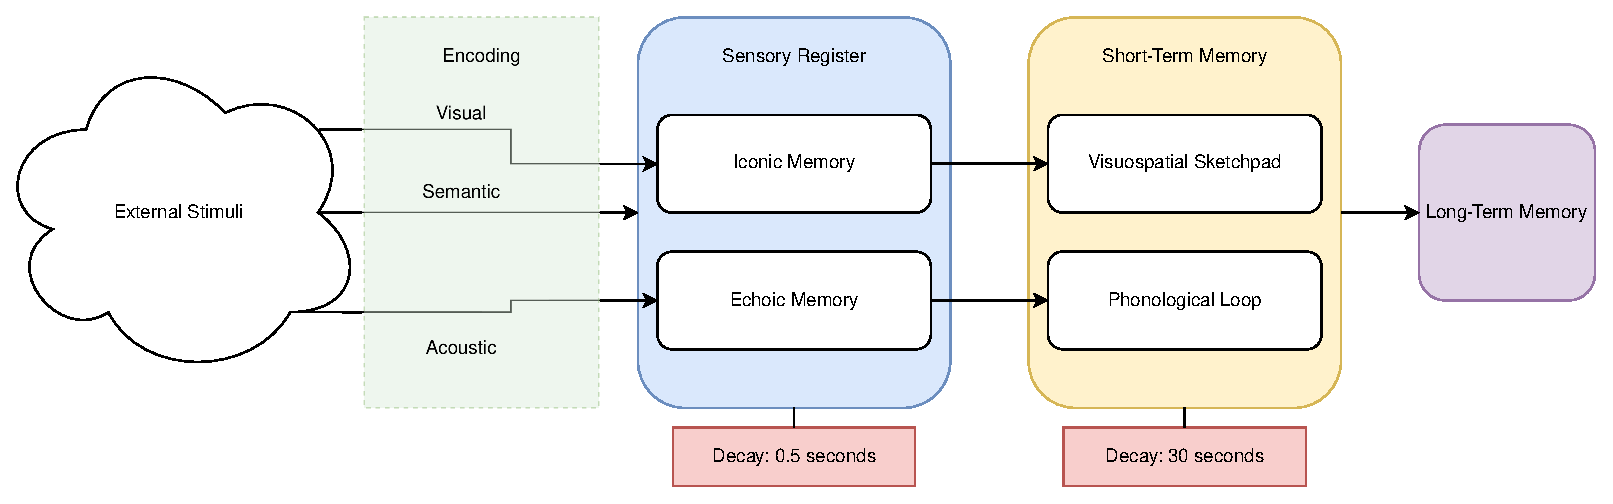
\includegraphics[width=\textwidth]{02.Background/atkinson.eps}
    \caption{The Atkinson-Shiffrin Multi-Store Model}
    \label{fig:atkinson}
\end{figure}

As shown in Figure \ref{fig:atkinson}, the Atkinson-Shiffrin Multi-Store Model states that humans perceive information through external stimuli, and that information is encoded as three different types of stimulus. \textbf{Visual} encoding encodes information in pictures and diagrams, \textbf{Semantic} encoding encodes information in words and their meanings, while \textbf{Acoustic} encoding encodes information in sounds. This encoded information is processed by the sensory register. If attention is paid to this information, it travels into short-term memory, otherwise it decays within half a second and is forgotten. For information to progress from short-term to long-term memory, a process of repetition called maintenance rehearsal is necessary \cite{multi_store}, in which the information is repeated within the learner's mind. For visually encoded information, this could be through repeated visualisation of diagrams or patterns in what the learner sees on a screen, while for acoustically encoded information this is achieved through the learner playing back the soundbite in their head (phonological loop). A key take-away from this memory model is that human brains process different information encodings independently, meaning that even if one encoding type is saturated with information, additional information can still be conveyed to the learner using an alternative encoding method. 

In its current form, Issie encodes information about the digital circuit both visually (circuit diagram, error highlighting etc.) and semantically (error messages, simulation outputs). No information is encoded acoustically, however outside of chimes for errors there is not much scope for implementation of sounds. Furthermore, students will receive plenty of auditory information in the form of teaching from lab assistants and conversation with their peers. Any extensions added to Issie by this project should therefore focus on conveying information to users through a combination of diagrams with appropriate annotations and informative text.

\subsection{Educating Engineers} \label{subsec:educating_engineers}
As a tool for teaching Digital Electronics, Issie's primary user base is engineering students. Therefore, there is value in exploring trends in how engineers learn best, and tailoring Issie's design and structure to align with these trends.
In 1992, Fleming and Mills proposed that there were four categories of how students learned. These are \textbf{visual}, \textbf{auditory}, \textbf{reading/writing}, and \textbf{kinesthetic} \cite{Fleming1992}. Most learners will learn using all of these methods, however will exhibit a preference towards one or two. Studies have shown that engineers have a preference towards visual and kinesthetic learning techniques \cite{vark_engineers}. The visual aspect means that engineers prefer information be conveyed to them through diagrams, patterns, and highlighted meaningful symbols. On the other hand, the kinesthetic aspect means that engineers prefer to learn through demonstrations, simulations, and their own experiences. The existence of practical lab sessions and Issie itself lends itself to a focus on kinesthetic learning; students explore concepts they have been taught about in lectures by building and simulating combinational logic. Therefore, the results of the VARK survey concur with the current teaching style in the EEE Departement at Imperial College. Currently, Issie has an interactive diagram with highlighting (visual encoding), as well as simulators for testing logic and general experimentation (kinesthetic learning). Thus, it can be said that Issie in its current form is fit for its purpose: educating engineers. In turn, any extensions added to Issie by this project should continue this trend of visual and kinesthetic learning, but while also taking care to not overload the users' sensory register and short-term memory.

\subsection{Cognitive Theories of Self Efficacy and Constructivism} \label{subsec:self_efficacy}
There are more factors that contribute towards an effective learning experience than just the conveyance of information. The learning process must be structured in such a way that students remain motivated while learning complex concepts. A ten-year longitudinal study \cite{motivation} found that there is a significant correlation between students who are motivated, therefore having high self-confidence, and academic attainment. Therefore, while developing educational tools like Issie, an emphasis must be placed on communicating information to students in such a way that they retain the belief that they can successfully learn the content. This approach aligns well with the theory of constructivism in education, which seeks to educate students by having them discover knowledge intuitively in contrast to traditional methods in which a student is considered an 'empty vessel' waiting to be filled up by a teacher \cite{construct}. The rationale behind the theory is that this self-discovery of knowledge will build a stronger conceptual understanding of what is being learnt. Constructivism aligns well with teaching styles that suit kinesthetic learners, as both approaches focus on students learning through their own experiences. Engineers tend to be kinesthetic learners, therefore, this project should aim to improve Issie in such a way that students are able to interactively and iteratively build their understanding of digital electronics and circuit design by themselves.

\section{Combinational Logic}
Combinational logic is a type of digital logic in which the output of the logic is a pure function of its present inputs \cite{comblog_wiki}. This means that combinational logic is memoryless; it is not affected by any previous outputs. This is in contrast to sequential logic, for which the output is dependent on present input values and some internal state derived from previous outputs.

\subsection{Visualising Logic with Boolean Algebra}
The aforementioned pure function which maps inputs to outputs can be written as a Boolean expression. A Boolean expression, much like traditional mathematical expression, features a set of input terms combined using operators. There exist three fundamental Boolean operators \cite{gregg_boolean}:
\begin{itemize}
    \item[] \textbf{NOT}, a unary operator which outputs the inverse of the input.
    \item[]\textbf{AND}, a binary operator which outputs HIGH when both inputs are HIGH and LOW otherwise. Denoted by 
    \item[] \textbf{OR}, a binary operator which outputs HIGH when either of the inputs are HIGH, and LOW otherwise
\end{itemize}
Other Boolean operators, such as \textbf{NAND}, \textbf{NOR}, and \textbf{XOR} also exist, but can be defined using a combination of the three fundamental operators.
Therefore, the first and most basic way of visualising combinational logic is simply through writing the Boolean expression which represents it. However, it can be difficult to quickly understand what some logic does using just Boolean expressions. Take for example the following Boolean equation for output $Y$, derived from inputs $S$, $A$, and $B$:
\begin{equation}
       Y = \overline{S}.A + S.B
       \label{equ:MuxEq}
\end{equation}
While the operations performed are clear, it may not be very clear on first inspection to an inexperienced student what the expression actually achieves. Furthermore, Boolean expressions grow in complexity as schematics become larger, making them even tougher to understand at a glance.

\subsection{Visualising Logic with Schematic Diagrams}
Schematic diagrams give the hardware representation of the combinational logic, and are the primary way of creating and visualising combinational logic in Issie. At their simplest, they consist purely of logic gates; these gates each correspond to a Boolean operator. However, in practice (and Issie) schematics are at a slightly higher-level, with certain combinational components (which can be built from gates) pre-created for the user. For example, Equation \ref{equ:MuxEq} represents a 2-bit Multiplexer, which is a component available in Issie's catalogue. The recall of stored knowledge due to the visual stimulus of the multiplexer component on the diagram is much more likely compared to the semantic stimulus of the Boolean expression. However, as a schematic increases in size, the number of components may become so large that holding all of the visual stimuli in short-term memory is unfeasible. Issie combats this by letting users modularise their schematic through hierarchical custom components. Alongside decreasing schematic size and repeated logic, this feature actually aims to teach students the technique of modularising their work (whether that is a schematic or code), and its advantages. These advantages \cite{arm_modular} include efficient development, easier dubugging, and logic reuse. However, as mentioned in the Project Motivation, hierarchical components are not always effective (particularly if badly named and organised), leaving a opportunity for improvement through complementary visualisation techniques. 

\section{Truth Tables} \label{subsec:TruthTables}
A truth table represents a given combinational logic function; featuring all input combinations on the left, and their corresponding output(s) on the right. As the truth table maps all possible inputs to their output, it is trivial to look up the behaviour of the logic in a given scenario. A very basic example is the truth table for the Boolean \textbf{AND} operator, shown in Table \ref{tab:And_TT}.

\begin{table}[h!]
    \centering
    \begin{tabular}{c|c||c}
     \textbf{A} & \textbf{B} & \textbf{C} \\
     \hline
     0 & 0 & 0  \\
     0 & 1 & 0  \\
     1 & 0 & 0  \\
     1 & 1 & 1
    \end{tabular}
    \caption{Truth Table for the Boolean AND operator ($C = A.B$)}
    \label{tab:And_TT}
\end{table}

Given that a truth table defines some logic using an exhaustive set of examples, it could be said that truth tables are ideal for kinesthetic learners. This exhaustive property can also be used to test for logical equivalence. Suppose the claim is made that two schematics, with one schematic featuring far fewer components than the other, are logically identical. Equivalence could be confirmed by simply checking if the truth tables for the two schematics are the same. 

However, a disadvantage of using truth tables to visualise combinational logic is that they can very rapidly grow in size. For logic with $n$ single-bit inputs, the number of rows in the associated truth table is $2^n -1$. For multi-bit inputs this number would grow even larger. Thus, Issie schematics with a large number of inputs would result in very long truth tables, which would likely intimidate the user. The size of generated truth tables could be reduced by filtering them based on user selections, or through truth table reduction methods.   

\subsection{Reduction using Don't Cares} \label{subsec:dcbackground}
A "Don't Care" term in a truth table can mean different things based on it's positioning. It is more commonly seen on the right-hand side of a truth table, signifying that an output for a given input combination is invalid or has no use \cite{1969logic}. This information is often used when attempting to simplify Boolean expressions using Karnaugh maps. On the other hand, a Don't Care term in an input row signifies that the particular input has no effect on the eventual output of the logic for that combination. These \textit{Don't Care inputs} can be found through logic minimisation, of which there are numerous techniques ranging from the aforementioned Karnaugh Maps \cite{kmapbook} to heuristic-based tools like Espresso \cite{espresso}. The latter is very effective at reducing large circuits efficiently, and would therefore appear to fit the needs of the project well. An example of the reduction can be seen in Table \ref{tab:muxTTs}, where the eight row exhaustive truth table (\ref{subfig:muxTT_standard}) is reduced to two rows (\ref{subfig:muxTT_dc}). However, Espresso and other common minimisation techniques treat their inputs and outputs as single-bit Boolean values which are either \codestyle{ON}, \codestyle{OFF}, or \codestyle{DC} -- corresponding to 1, 0 and Don't Care \cite{espressoinputs}. Multi-bit IOs are broken into their constituent bits. In Table \ref{subfig:muxTT_dc}, only HIGH outputs are shown -- this works when it can be assumed that all other input combinations yield 0. This approach aligns well with industrial applications, where signals on wires can only be HIGH or LOW, and there is value in reducing to the form which requires the fewest gates.  On the other hand, Issie is an educational application where inputs and outputs can have more than two values, and focus is more on semantics and understanding rather than the most cost-efficient hardware design. Therefore, such minimisation would not integrate well with Issie's existing implementation of multi-bit IOs.

In order to implement DC reduction in Issie, a suitable algorithm will have to be written which supports multi-bit inputs. One possibility may be analysis of redundancies in the existing truth table. For example, in the full truth table, the first and third row both have an output value of 0, with the only difference being the change in the value of $B$. Given that $B$ can only take two values, this shows that when $A=0$ and $S=0$, the value of $B$ does not affect the output - therefore we "don't care" about B. Rows one and three can therefore be collapsed into one row, with the entry for the $B$ column being replaced with an "X". This process can be repeated until all such row combinations have been collapsed. The results from this process can be seen in Table \ref{subfig:muxTT_dc_zeros}. The length of the truth table has been reduced by 25\%, and the actual semantic function of what the multiplexer does is much clearer as well. This table is however, much larger than the reduced table generated by Espresso, indicating that it may not work well with larger schematics.

\subsection{Algebraic Truth Tables}
While reduction with Don't Cares is useful, neither implementation of it is ideal. Industry-style minimisation doesn't fully align with Issie's implementation, while custom algorithms may not be reduce the table enough. Additionally, Don't Care reduction cannot simplify relationships which involve all inputs, such as arithmetic. A viable alternative is an Algebraic Truth Table; these are often found on component datasheets \cite{timux} and have the task of summarising the behaviour of the circuit in a concise and readable format.  One such example is shown in Figure \ref{fig:datasheet}, which is an excerpt from a datasheet for a three-input multiplexer. H and L are equivalent to 1 and 0, but the terms of form $I_x$ in the table are algebraic values representing inputs. The select signals ($S2,S1,S0$), which actually control the circuit behaviour are still numeric.

\begin{figure}[h]
    \centering
    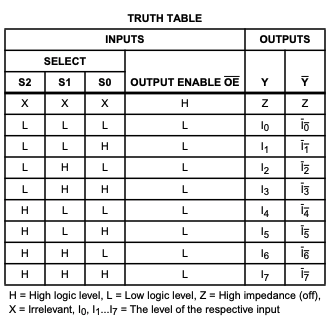
\includegraphics[width=0.5\textwidth]{02.Background/datasheet.png}
    \caption{Algebraic Truth Table in Datasheet for a Three-input Multiplexer \cite{timux}}
    \label{fig:datasheet}
\end{figure}

Table \ref{subfig:muxTT_alg} shows what the corresponding algebraic truth table would look like for the running example in this section.
$A$ is propagated to the output when the selection input ($S$) is low, and $B$ is propagated when $S$ is high. This clearly describes a two-input multiplexer. Having functionality which could create similar tables for user-created schematics, with support for more complex algebraic operators would likely be useful. This is because algebraic truth tables carry far more semantic information in a much smaller visual space, meaning that a students' sensory register is less likely to be overloaded.

\begin{table}[h]
    \centering
    \subfloat[Full Truth Table]{
    \label{subfig:muxTT_standard}
    \begin{tabular}{c|c|c||c}
     \textbf{A} & \textbf{B} & \textbf{S} & \textbf{OUT} \\
     \hline
     0 & 0 & 0 & 0 \\
     0 & 0 & 1 & 0 \\
     0 & 1 & 0 & 0\\
     0 & 1 & 1 & 1\\
     1 & 0 & 0 & 1\\
     1 & 0 & 1 & 0\\
     1 & 1 & 0 & 1\\
     1 & 1 & 1 & 1\\
    \end{tabular}}
    \medskip
    \subfloat[DC Reduced \\(Inc. Zeros)]{
    \label{subfig:muxTT_dc_zeros}
    \begin{tabular}{c|c|c||c}
     \textbf{A} & \textbf{B} & \textbf{S} & \textbf{OUT} \\
     \hline
     0 & X & 0 & 0 \\
     X & 0 & 1 & 0 \\
     X & 1 & 1 & 1\\
     1 & X & 0 & 1\\
     0 & 0 & X & 0 \\
     1 & 1 & X & 1
    \end{tabular}}
    \medskip
    \subfloat[DC Reduced \\(Espresso)]{
    \label{subfig:muxTT_dc}
    \begin{tabular}{c|c|c||c}
     \textbf{A} & \textbf{B} & \textbf{S} & \textbf{OUT} \\
     \hline
     1 & X & 0 & 1 \\
     X & 1 & 1 & 1
    \end{tabular}}
    \medskip
    \subfloat[Algebraic Truth Table]{
    \label{subfig:muxTT_alg}
    \begin{tabular}{c|c|c||c}
     \textbf{A} & \textbf{B} & \textbf{S} & \textbf{OUT} \\
     \hline
     A & B & 0 & A \\
     A & B & 1 & B
    \end{tabular}}
    \caption{Truth Tables for a 2-bit Multiplexer}
    \label{tab:muxTTs}
\end{table}


\section{An Overview of Issie's Technology Stack} \label{sec:techstack}

The reasoning and process behind the decisions made for Issie's technology stack can be found in Marco Selvatici's dissertation on DEFlow, the predecessor to Issie \cite{marco_diss}. This section describes the technology stack, and evaluates and reaffirms why Issie's technology stack is well suited.

\subsection{Programming Language} \label{subsec:fsharp}
Issie is written in F\fsharp, an open-source, cross-platform, interoperable programming language for writing succinct, robust and performant code \cite{fsharp}. It is functional-first; meaning that it contains many features found in functional languages and encourages a functional programming style while also allowing programmers the flexibility to use the programming styles of other paradigms. Pure functional programming languages adopt a philosophy of declarative programming and immutable data; data values cannot be updated after initial assignment, and functions take this data as input and map it to output data. These functions are deterministic, meaning that their output is solely dependent on the value of their inputs and that there is no internal state affecting the behaviour of the function. This differs from the more common imperative style of programming where code is treated as a sequential list of instructions which mutate program data/state. The deterministic nature of functions in pure functional programming makes them very easy to understand, as operations on data have no side-effects and are therefore very easy to track. Not only does this make debugging easier, but it leads to fewer overall bugs in the code. A large-scale study of programming languages and code quality on Github \cite{functionaldebug} found that "Functional languages have a smaller relationship to defects than other language classes, whereas procedural languages are either greater than average or similar to the average." The study also found that the "Functional-Static-Strong-Managed" class of languages (i.e. languages that are functional, statically and strongly typed with in-built memory management) are  less likely than average to result in defect-fixing commits on Github.
While not a part of the study, F\fsharp does belong to this class of languages, and is therefore a wise choice of programming language for Issie. F\fsharp features a Hindley-Milner type system, which has a provably sound type inference algorithm \cite{hm_typesis}. Type inference allows for F\fsharp to be statically typed while eliminating the need for type annotations in the code. This results in clean-looking and succinct code while still maintaining the benefits of static typing.  Furthermore, as types can be inferred on the fly by IDEs such as Visual Studio, it is much easier for the programmer to track the correctness of the program. 

\begin{wrapfigure}{l}{0.5\textwidth} 
  \begin{center}
    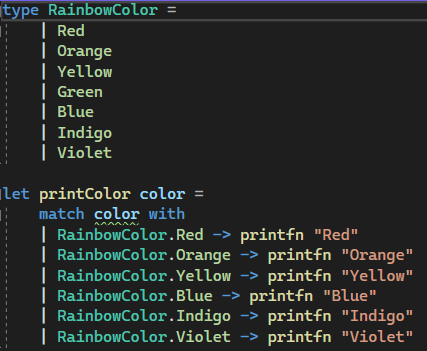
\includegraphics[width=0.40\textwidth]{02.Background/patternmatch.png}
  \end{center}
  \caption{An example of incomplete Pattern Matching in F\fsharp, with a warning from the compiler}
  \label{fig:patternmatch}
\end{wrapfigure}

One such example is found when pattern matching, as seen in Figure \ref{fig:patternmatch}. The function \codestyle{printColor} takes as input some colour of the rainbow (type \codestyle{RainbowColor}) and prints the colour. \codestyle{RainbowColor} is an F\fsharp Discriminated Union (DU) type \cite{dutypes}, where the data stored in the value is not fixed; it can be one of several distinct options. DU types have many applications, ranging from representing valid and error cases to small object hierarchies.  The type system allows for the IDE to first infer the type of the variable \codestyle{color}, and then realise that the pattern match does not cover the DU case for when \codestyle{color} is Green. Mousing over the warning line in Visual Studio gives the following message: "Incomplete pattern matches on this expression. For example, the value 'Green' may indicate a case not covered by the pattern(s)." Such hints are immensely useful for the programmer. The advantage of such checks being performed before and at compile-time is that it decreases the number of errors at run-time, which tend to be more disruptive.

F\fsharp also helps protect against runtime errors through the use of Monadic types. Sometimes, certain actions in a program may need to return \textit{nothing}, such as an unsuccessful lookup in a Map/Dictionary or if there is an absence of some data. Usually such messages are communicated within the program using either exceptions or NULLs which have to be caught and handled. If not tracked and handled appropriately, NULLs in particular can lead to some very nasty and hard-to-debug runtime errors. F\fsharp allows programmers to minimise the use of exceptions and avoid the use of NULLs using the \codestyle{Option} and \codestyle{Result} types. The \codestyle{Option} type can take the value \codestyle{Some <type a>} or \codestyle{None}, giving the programmer a safe way to indicate nothing without using NULLs. The \codestyle{Result} type can reflect success (\codestyle{Ok <type a>}) or failure (\codestyle{Error <type b>}), giving the programmer a safe way to propogate errors through their code without raising exceptions or returning NULL. 

While F\fsharp has the many features and benefits of pure-functional languages and strongly encourages the programmer to use them, it is an impure functional language and does allow the programmer to use other styles of programming. For example, mutable state in functions is allowed by the use of the \codestyle{mutable} keyword upon definition. This allows flexibility; programmers can use the default functional style in most places, and can selectively choose where to introduce functionally impure constructs such as mutable state. An example of this in Issie is the \textit{FastSimulation} used by the Step Simulator, which uses mutable arrays to represent the value of component inputs/outputs at different clock cycles.

As most of the features mentioned in this section are either unique to or far better implemented in F\fsharp compared to other common app development languages such as JavaScript or Python, and that F\fsharp belongs to the most bug-free class of languages, it can be said that Issie's choice of programming language is apt and ideal.

\subsection{Ecosystem} \label{subsec:ecosystem}
While originally built as a language for the .NET framework, built to run on the Microsoft Common Lanugage Runtime (CLR) \cite{clr_mag}, F\fsharp can also execute in Javascript environments through the use of third-party trans-compilation tools \cite{fableio}. Therefore, F\fsharp can be used to build desktop applications using .NET, as well as Javascript web apps. Issie is built using the latter method; F\fsharp code is compiled to JavaScript, which is executed in a desktop environment through Electron. This section describes the chosen tools in this process, and the reasoning behind those choices.

\subsubsection{Electron}
Electron \cite{electrondocs} is a framework for building desktop applications using JavaScript, HTML, and CSS. Electron comes bundled with the open-source Chromium browser and Node.js, a runtime environment that lets JavaScript code execute outside of a browser. Using these, Electron enables web apps to run locally on the user's machine outside of a web browser, akin to a native program. The advantage of this approach is that a developer can create a cross-platform application without any experience of programming native applications for any platform. On the other hand, pure native desktop applications often require differing codebases if multiple platforms are to be targeted \cite{webapps}; this is a far more labour-intensive approach which also requires a wider skill set. Common native desktop application technologies, such as UWP and WPF, have a much steeper learning curve compared to Electron as well \cite{mustdecisions}. Given that Issie is maintained by various students over time, an ecosystem that allows for easy cross-platform development with a relatively shallow learning curve is preferable, making Electron well suited for Issie's ecosystem.

However, potential issues with Electron must also be discussed. As Electron apps bundle Chromium and Node, they are often quite large. Additionally, due to the use of the RAM-intensive Chromium browser, Electron apps tend to use more memory than other similar applications \cite{roryok}. This could lead to decreased performance on low-end hardware. Electron is also dependent on a large amount of open-source code, and web apps are often very reliant on Node dependencies, which can change at any time. This reliance could also be perceived as a weakness.

However, despite some of its shortcomings, Electron is still a good fit for Issie's use case. Issie in its current form is performant, responsive, and stable; implying that the performance issues with Electron have not affected Issie significantly enough for there to be notable issues. The advantage of easy cross-platform development, as well as good integration with Fable (which allows F\fsharp to be used as the programming language), outweighs the risks posed by potential Node dependency issues, as well as a larger app footprint.

\subsubsection{Fable}
While Electron provides a convenient framework for building cross-platform applications, it requires a JavaScript codebase. JavaScript is a weakly and dynamically typed imperative language - making it a sub-optimal choice for the development of Issie. The gap between development and deployment is bridged by \textbf{Fable} \cite{fableio}, a compiler that brings F\fsharp to the JavaScript ecosystem. Fable compiles F\fsharp to clean JavaScript code which can run under Electron. Fable also includes bindings for React \cite{reactjs}, a highly performant JavaScript library for building user interfaces; this allows Issie's F\fsharp code to create React elements which Fable will compile to their respective JavaScript implementations.

\subsection{User Interface and Rendering}
A well-written and structured Graphical User Interface (GUI) is an essential component of any application, but it becomes even more vital in the context of an application like Issie which prioritises an interactive and intuitive interface. In Issie, most of the user's interaction with the program is done using the mouse; clicking, dragging, and hovering. This means that the UI code must be able to handle a constant stream of pseudo-random mouse events and deal with them quickly and appropriately. It must also be maintainable and extensible to easily allow for more functionality to be added over time. This section describes the workings of Issie's UI framework, as well as the reasoning behind the decision to choose the framework.

\subsubsection{Elm, Elmish, and MVU}
The Elm Architecture \cite{elmarch}, also known as the MVU Architecture, is a pattern for creating interactive programs which emerged from the Elm programming language. Elm \cite{elm} is a purely functional language for creating websites and web apps. Elm compiles to JavaScript - this is similar to how using F\fsharp with Fable allows functional F\fsharp code to be compiled to JavaScript for a web app. Issie uses the Elmish library \cite{elmishdocs}, which brings Elm's MVU architecture to F\fsharp and integrates well with Fable, enabling Issie's smooth and robust GUI.

The MVU architecture gains its name from the three parts it splits the UI code into:
\begin{itemize}
    \item[] \textbf{Model:} A data structure which stores the state of the application. In Issie this is a very large record, containing lots of information ranging from the results of a simulation to which components are selected and highlighted.
    \item[] \textbf{View:} A pure function which specifies how the information in the model (application state) should be displayed to the user. The developer writes a function to turn the model into HTML/CSS equivalents, and Elm (or Fable if using F\fsharp with Elmish) converts this to actual HTML/CSS and renders it. 
    \item[] \textbf{Update:} A way to update the application state triggered by events such as user input. These events are communicated within the program using \textit{messages}, which are triggered by the user interacting with the GUI. The update function is a  pure function which accepts two parameters, the incoming message and the current model. It then interprets the message and returns an updated version of the model. 
\end{itemize}

An initial Model is specified in the code, which is rendered by the View function on application startup. The user can then interact with the application - each interaction will generate a message which is passed to the update function. The update function processes this message and, if required, will return an updated model which reflects the effects of the interaction. On its next invocation, the View function will render this updated application state, showing the user the result of their interaction.

The MVU Architecture has numerous strengths, many of which make it suitable for use in Issie. It's structure, based on an immutable Model with deterministic (pure) View and Update functions, means that data flows in only one direction through the whole application, while events which warrant a change in the application state are clearly marked as messages. This making the rendering process easier to understand for the programmer \cite{mvuthesis}, meaning that more time is spent writing useful code instead of debugging. This is unsurprising given that Elm, like F\fsharp, is a functional language, and therefore belongs to the "Functional-Static-Strong-Managed" class of languages mentioned in Section \ref{subsec:fsharp}. F\fsharp also has features which integrate well into the MVU architecture, strengthening it further. One such example is F\fsharp's strict compile order, which helps avoid cyclic references between view subfunctions \cite{mvuthesis}. Altogether, the MVU architecture is a good fit for Issie, improving the developer experience while delivering a performant UI.

On initial inspection, the design decision of having a View function which repeatedly re-renders the Model every time there is some update appears inefficient. This would be the case if Elm (and other implementations of MVU) used the traditional process for rendering a web page/app.
This traditional process for rendering HTML is shown in Figure \ref{fig:tradDOM}. The HTML is parsed and a DOM (Document Object Model) is constructed; this is a tree representation of the HTML. Whenever the website/web app state changes, certain parts of the generated HTML change too. The DOM tree must be updated to reflect these changes, however this is often a slow process for large web apps with a large number of nodes in the DOM tree, resulting in the UI appearing sluggish. Elm combats this by using an intermediate \textbf{Virtual DOM}, a lightweight and optimised version of the main DOM tree on which operations are cheap. As shown in Figure \ref{fig:virtualDOM}, Elm exposes this virtual DOM to the programmer, who specifies how the state should be viewed in the View function. For each change of state, a new virtual DOM is constructed and compared to the previous virtual DOM. Through this, Elm can determine the exact change to the UI. Both the construction and comparison are fast due to the lightweight nature of the virtual DOM. Elm repeats this process for multiple changes to the UI, creating a batch of updates to be performed on the actual DOM tree at once. This method significantly reduces the per-update penalty for updating the DOM, allowing for efficeint re-rendering of the program state. This improves the performance of the web app. Another advantage of this method is that the task of efficiently updating the DOM is abstracted away from the programmer, leaving them with only the task of specifying how their website or web app should look.

\begin{figure} [h]
    \centering
    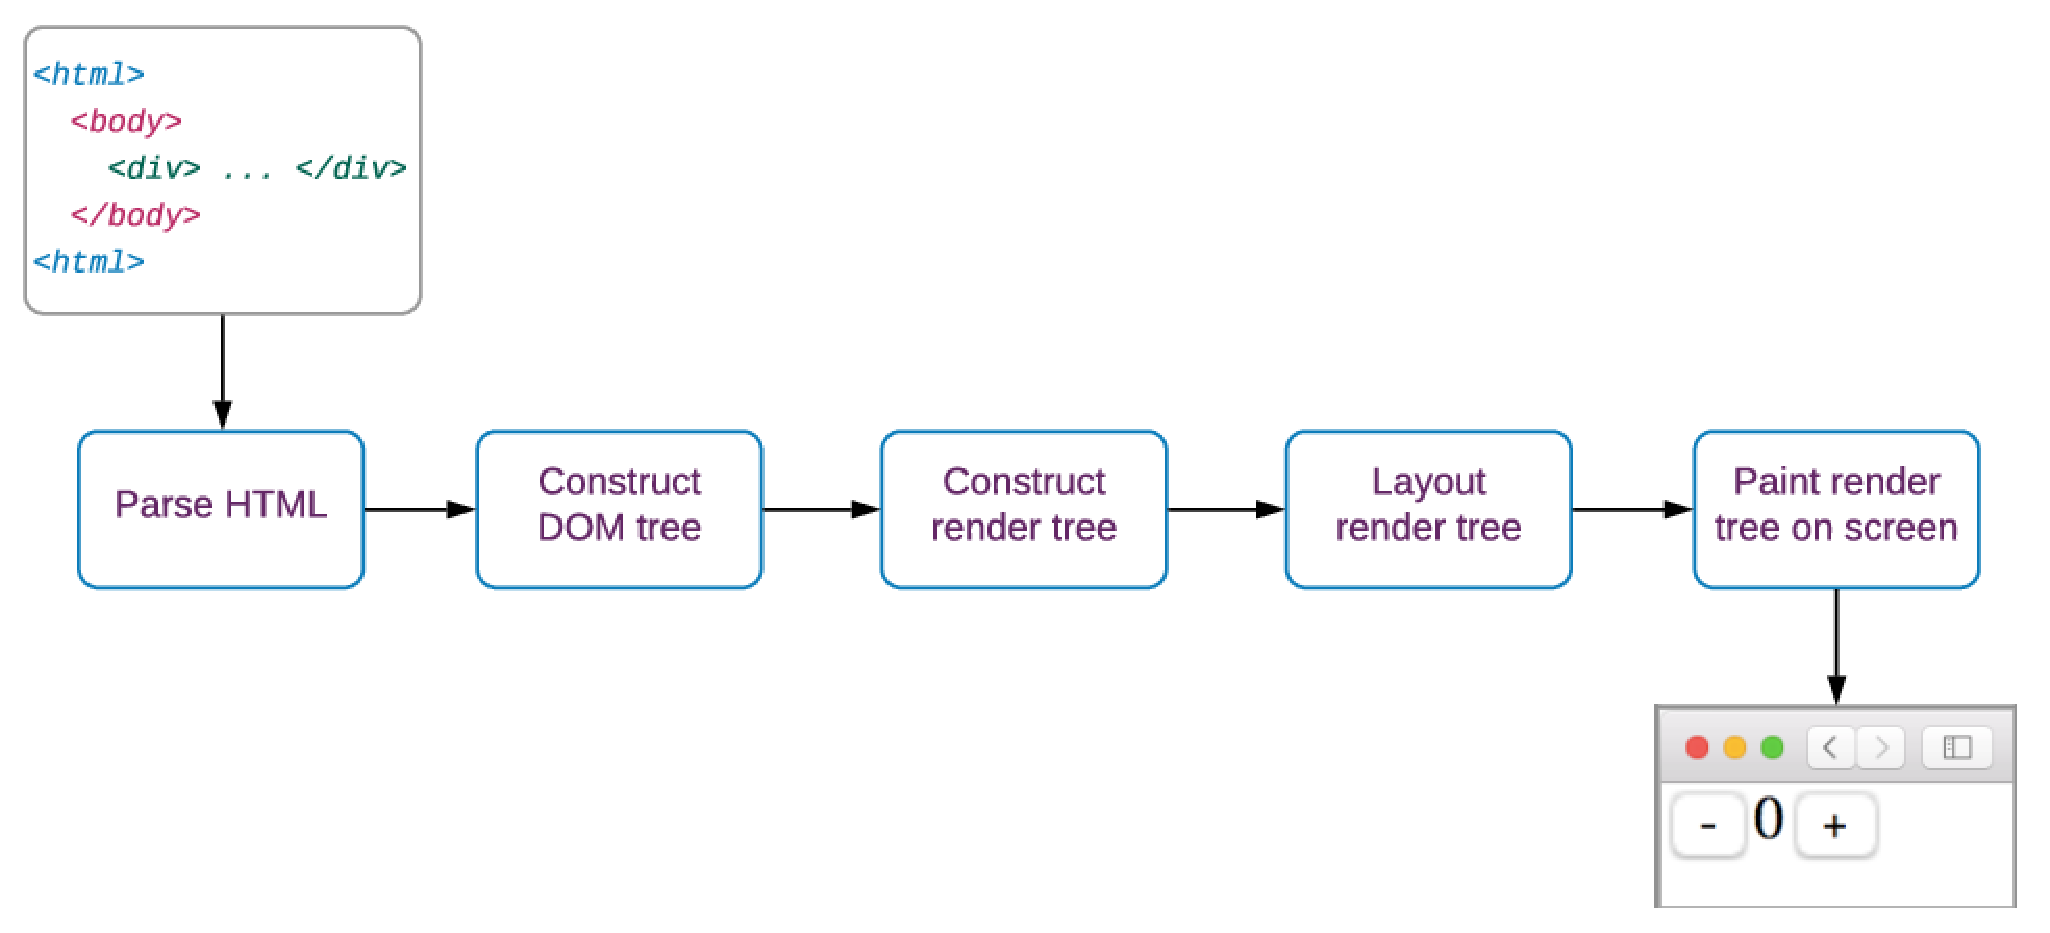
\includegraphics[width=\textwidth]{02.Background/traditionalDOM.eps}
    \caption{How browsers traditionally render HTML using a DOM \cite{virtualdom}}
    \label{fig:tradDOM}
\end{figure}

\begin{figure} [h]
    \centering
    \includegraphics[width=\textwidth]{02.Background/elm-virtual-dom.eps}
    \caption{The Elm Architecture \cite{virtualdom}}
    \label{fig:virtualDOM}
\end{figure}

\subsubsection{React}
React, as mentioned earlier, is a library for building user interfaces. In the Issie project, Elmish uses React for rendering the UI due to its efficient virtual DOM. Thus, the virtual DOM mentioned previously is actually the React Virtual DOM, which is a tree of React Elements. React Elements are simple objects, and are therefore cheap to create \cite{reactrender}, meaning that operations on the React DOM are computationally inexpensive. The View function returns a React Element which shows the current state of the UI. React improves the performance of an application by only re-rendering elements when necessary. The React equivalent of the process mentioned previously where virtual DOMs are compared to find UI changes is called \textit{Reconciliation} \cite{reactrender}.

React also provides a further method for increasing performance: memoization \cite{reactcache}. Memoization is most useful when working with components whose state is partially dependent on computationally intensive calculation. Under traditional React, this value would be re-calculated on every render, even if it had not changed. This increases the amount of time each render takes. An example of this would be the result of the addition of two very large numbers ($a + b$), which is a very CPU intensive task. Memoization combats this by caching the previous value of the computation and only performing the calculation whenever $a$ or $b$ changes. Issie already uses some memoization in its code for the Step Simulator: after a sheet is simulated for the first time the simulation is cached. If the sheet hasn't changed the next time a simulation is started, the cached simulation is used instead of building a new one, increasing performance. 
\subsubsection{Fulma} \label{subsec:fulma}
Fulma \cite{fulmaio} is an F\fsharp library which provides a wrapper around Bulma \cite{bulmaio}, an open-source CSS framework which provides ready-to-use front-end components for building responsive web interfaces. Fulma brings these components to F\fsharp for use with Fable React. React components such as buttons, forms, and tables can easily be specified in the F\fsharp code using the functions provided by Fulma. Listing \ref{lst:fulmatable} shows the F\fsharp code for generating a table using Fulma, while Figure \ref{fig:fulmatable} shows the rendered table.

\begin{lstlisting}[language=FSharp, caption={Simple F\fsharp code for generating a table with Fulma \cite{fulmatable}}, captionpos=b, label={lst:fulmatable}]
    Table.table [ Table.IsBordered
              Table.IsNarrow
              Table.IsStriped ]
    [ thead [ ]
        [ tr [ ]
             [ th [ ] [ str "Firstname" ]
               th [ ] [ str "Surname" ]
               th [ ] [ str "Birthday" ] ] ]
      tbody [ ]
        [ tr [ ]
            [ td [ ] [ str "Maxime" ]
              td [ ] [ str "Mangel" ]
              td [ ] [ str "28/02/1992" ] ]
          tr [ ClassName "is-selected" ]
             [ td [ ] [ str "Jane" ]
               td [ ] [ str "Doe" ]
               td [ ] [ str "21/07/1987" ] ]
          tr [  ]
             [ td [ ] [ str "John" ]
               td [ ] [ str "Doe" ]
               td [ ] [ str "11/07/1978" ] ] ] ]
\end{lstlisting}

\begin{figure} [h]
    \centering
    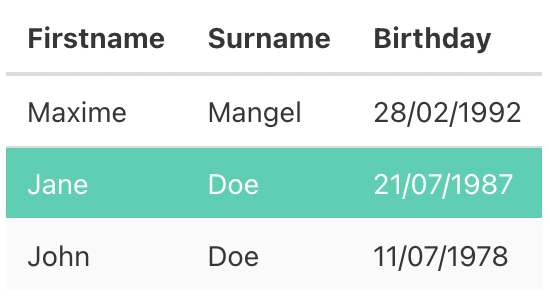
\includegraphics[width=0.5\textwidth]{02.Background/Fulma Table.png}
    \caption{Fulma Table Example}
    \label{fig:fulmatable}
\end{figure}


\subsection{Overview}
\begin{figure} [h]
    \centering
    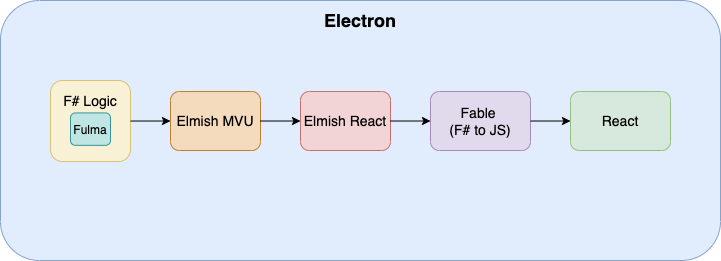
\includegraphics[width=\textwidth]{02.Background/Stack.png}
    \caption{An Overview of Issie's Technology Stack}
    \label{fig:techstack}
\end{figure}
We can bring the above sections together to get an overview of Issie's Technology Stack, which is presented in Figure \ref{fig:techstack}. The core logic of the Issie application is written in F\fsharp, with a structure which allows for adoption of the MVU architecture. Within the View function, using libraries like \codestyle{Fable.React} and \codestyle{Fulma}, HTML and React components can be specified. The \codestyle{Elmish} library provides the MVU framework and methods for bringing together the Model data structure, View function, and Update function. A virtual DOM is necessary for an MVU application because it allows the application to frequently re-render its state after each update in an efficient manner. Due to its reliable and performant implementation of a virtual DOM, the React framework is used for Issie. The library \codestyle{Elmish.React} handles the transition from the generic Elmish view to React, after which \codestyle{Fable} compiles all of this F\fsharp code to JavaScript for React to render. All of this runs within Electron, allowing Issie to run as a desktop application despite having the technology stack of a web app.

\section{Issie's UI} \label{sec:IssieUI}
\subsection{Overview and Evaluation}
In line with the core principles that state all features implemented in Issie should be \textbf{Obvious} and \textbf{Intuitive}, Issie's UI aims to be consistent and straightforward. Consistency in the UI helps constantly prove a user’s assumptions about the user interface right, creating a sense of control, familiarity, and reliability \cite{uiconsistency}. It also plays a crucial role in exposing all of the features of an application to the user -- this is because features which are accessed in an inconsistent manner may be missed or incorrectly understood by end users. The intuitive guidance provided by a consistent and straightforward UI means that students using Issie spend less time learning how to use it compared to other similar applications; at it's launch most students were able to get started within five minutes \cite{marco_diss}. With the limited amount of time in labs available, less time spent learning to use tools means more time spent on learning educational content.

Since its original release, more features have been added to Issie, such as the Waveform Simulator, with the UI being updated to accommodate these features. At the time of writing, the latest release version of Issie is version 3.0.0, released on 16th April 2022. Images of Issie's UI can be found in Appendix A. On launch, Issie gives the user the option to create a new project or open an existing one. A project consists of one \textbf{main} sheet, and any number of sub-sheets, which define reusable custom components. Figure \ref{fig:IssieSheetAnnotated} is an annotated screenshot of a sheet open in Issie. The UI can be split into the following sections, which are highlighted in different colours in Figure \ref{fig:IssieSheetAnnotated}.

\begin{itemize}
    \item[] \textbf{Traditional Menu Bar (Highlighted Red):} The traditional menu bar, consists of the "Edit" and "View" menus. It is not used to expose Issie's core features - instead, it is used to let the user do basic operations, such as zooming, copying and pasting etc. Many of these functions are duplicated through keyboard shortcuts or through the buttons in the bottom left of the sheet (undo, redo, copy, paste). The fact that Issie has two separate menus is a little strange, and it may be worth moving all functionality from the traditional menu bar to the top white menu bar. However, this is not an urgent cosmetic issue.
    \item[] \textbf{The Canvas:} The canvas is the central focus of the application - it is where the schematic is designed. Components are dragged onto the canvas, with red-dashed lines appearing to show when a component is aligned with a grid line. Components and connections on the canvas can be interacted with in many ways, such as hovering, clicking to select, and dragging to move.
    \item[] \textbf{Right Tabs Panel (Highlighted Green):} The panel on the right-hand side of the application provides the user with ways of (i) affecting the state of the canvas and (ii) gaining insight into the schematic itself. There are three tabs: the \textbf{Catalogue}, which lets users add new components to the canvas (users can hover on components for details); \textbf{Properties}, which lets users view and modify component properties like name and width, and \textbf{Simulation}, which opens the Step Simulator, giving users the option to start a simulation. Due to the Step Simulator requiring more display real-estate, the right panel widens when the Simulator tab is selected. When the Waveform Simulator is running, an additional fourth tab  appears in this section -- this makes the tab layout appear cramped.
    \item[] \textbf{Top Bar (Highlighted Blue):} In the first release of Issie, the white menu bar located at the top of the application contained controls to, (i) save the current sheet, (ii) Switch to another sheet in the open project, and (iii) Open another or create a new project. The filepath of the current project and sheet are also displayed. All of these elements were consistent - with the focus on interacting with files. A slight grievance with the "Project" and "Sheets" dropdown menus is that they are not closed by clicking elsewhere in the application, only by clicking on the menu again. Since then, an "Info" button has been added featuring information about Issie and a short user guide. While this is not necessarily consistent with the other elements in its vicinity, the top bar enables the "Info" button to have maximum visibility, something which a student requiring information may appreciate. One very inconsistent part of the UI is how the Waveform simulator is accessed. While most actions which analyse the schematic (e.g. Step Simulator) are accessed via the Right Tabs panel, the Waveform simulator is opened through a button on the top bar. This causes the previously unseen "WaveSim" tab to spawn in the right panel, and the panel boundary becomes draggable. The user can select the waveforms to view (Figure \ref{fig:IssieWSSel}) and then view the waveforms (\ref{fig:IssieWS}. The Waveform simulator's behaviour is inconsistent with that of the Step simulator:
    \begin{itemize}
        \item Step Simulator displayed in a wider, fixed-width panel. Waveform Simulator displayed with panel starting at regular width, but the panel can be manually resized by dragging.
        \item The user can start a simulation in the Simulation tab, and still interact with other tabs. This is not the case for the Waveform simulator, which locks the user in the WaveSim tab.
        \item Step Simulation started and ended with the same button, with a clear indication of how to end the simulation. There is no end/close button on the WaveSim tab when waveforms are being viewed. Instead, the user must press the "Edit List" button, which takes them back to the selection menu where there is a close button. This is very unintuitive.
    \end{itemize}
    \item[] \textbf{Buttons on bottom-left (Highlighted Yellow):} Undo, Redo, Copy, and Paste buttons. These are four common functions, and therefore it makes sense to have obvious and fast ways to access them. Useful to get started if the user is not familiar with keyboard shortcuts.
\end{itemize}

\subsection{Considerations when adding new features}
As discussed in the previous section, Issie's UI at time of launch was very intuitive and straightforward. However, when there are fewer features it is easier to condense the interfaces for them into a well structured and streamlined UI. The inconsistencies of the Waveform Simulator tell a cautionary tale of how new features can introduce impurities into an application's GUI. This project aims to add a whole new way of visualising logic (truth tables) to Issie, and given the saturated nature of the current UI, some redesigning may be necessary to accommodate all features.

\section{Combinational Logic Simulation in Issie} \label{sec:simulationbackground}
Currently in Issie, the users can gain an understanding of combinational logic by simulating it using the Step Simulator. Users provide values for each input to the logic, and can read the output almost instantly. This indicates high performance. Given that visualisation of combinational logic through truth tables is likely to require some form of combinational simulation, there is merit in exploring and understanding the implementation of the performant Step Simulator.

Figure \ref{fig:flowchartSim} provides an overview of Issie's process for building and running a Step Simulation. In this process, various checks must be performed; firstly the logic designed by the user must be verified to be syntactically correct, secondly the organisation of project files must be correct, and thirdly some Issie specific limitations (e.g. no cycles in combinational logic) must be enforced. Issie's simulation building process can be said to have three levels, with each level having an associated data structure which represents the schematic. These data structures are: the \textbf{Canvas State}, \textbf{Simulation Data/Error}, and a \textbf{Fast Simulation}. A set of checks are performed at each level, and only upon passing these checks can a schematic be transformed into the subsequent data structure.
If any of these checks fail due to an issue with the user's schematic, the simulation building process returns a \textit{SimulationError}, which tells the user what the error is and which components/connections are affected. A key takeaway from Figure \ref{fig:flowchartSim} is that the process of building a simulation is separate from the process of running it. During the \codestyle{FastSimulation} building process, the schematic is analysed, with components being placed into an appropriate order for combinational reduction. However, as the \codestyle{FastSimulation} data structure is mutable, the values of each input can be updated without having to rebuild the whole simulation. Therefore, the time taken simulating a different input combination is quite short, as only the reduction function has to be re-run to find the new outputs. 
This distinction between building a simulation and running it with different input values makes the existing Step Simulator an optimal choice for use in truth table generation, which will need to simulate multiple input combinations as fast as possible. 

\begin{figure}[h]
    \centering
    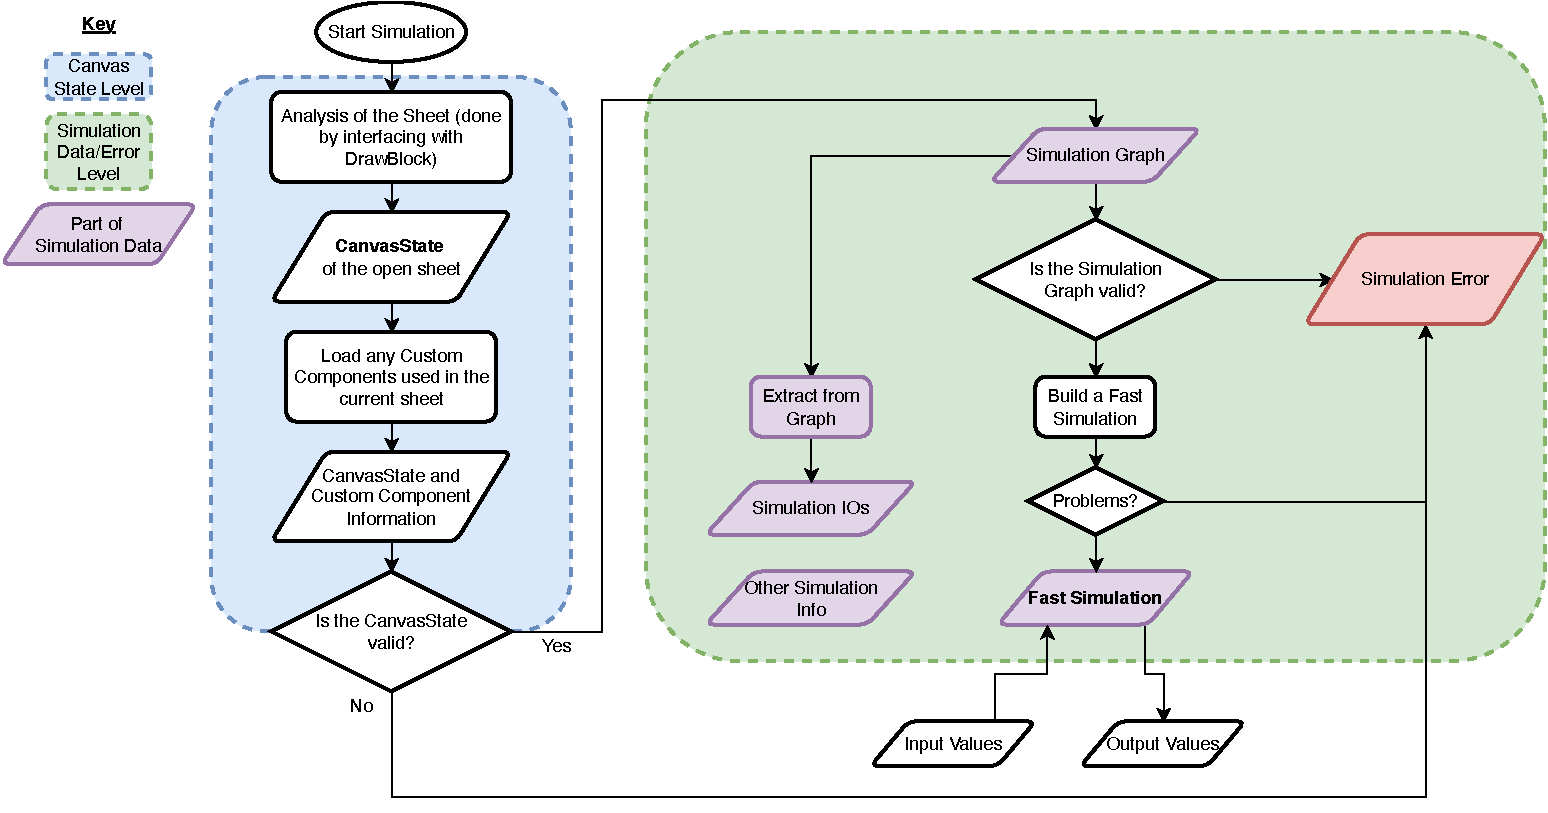
\includegraphics[width=\textwidth]{04.AnalysisDesign/IssieSim.pdf}
    \caption{An overview of Issie's Step Simulation}
    \label{fig:flowchartSim}
\end{figure}

\section{Effects of Application Performance on Users} \label{sec:perfeffects}
Interactivity is a key part of Issie, and one of the major contributors to perceived interactivity is the perceived responsiveness of an application \cite{interactiveWu}, which itself is often tied to application performance. Perceived responsiveness is relevant in systems where a user's "perceived control over the interaction process reflects their ability or confidence in performing related activities". Combining these findings with the cognitive theory of self-efficacy described in Section \ref{subsec:self_efficacy}, which proposes that academic performance is linked to perceived ability, indicates that perceived responsiveness is an important factor to consider when building an educational application. Robert Miller \cite{Miller1968ResponseTI} describes three classes of perceived responsiveness based on a computer's response time:
\begin{itemize}
    \item $\leq 100ms$: Perceived as instantaneous.
    \item $\leq 1s$: Noticeable but does not lose the user's attention.
    \item $\geq 10s$: Loses the user's attention.
\end{itemize}

Ideally, every interaction would be in the first class, however naturally certain tasks will take longer than others. In his paper, Miller investigates specific "Topics": examples of human-computer interaction, and examines the acceptable response time. A \textit{"Response to complex inquiry in tabular form"} (Topic 9) should return a complete response within 4 seconds, but a maximum delay of 2 seconds is preferred. This is particularly relevant to this project as it resembles the operation of calculating and presenting a Truth Table to the user. Therefore, it could be suggested that in order for the added Truth Table generation feature to have the maximum positive effect, generation should take less than 4 seconds in all cases, and ideally less than 2 seconds for simpler cases. By the same rationale, this time limit should also apply to complex operations on the truth table, such as reduction with Don't Cares or Algebra.
As mentioned in subsection \ref{subsec:educating_engineers}, engineers tend to be kinesthetic learners and therefore are likely to prefer tools which let them interactively experiment with what they are learning. Therefore, it can be proposed that increasing the responsiveness of Issie (which increases perceived interactivity), will lead to a better learning experience. 


\section{Agile Software Development}
Agile software development \cite{alma9955899676101591} is an iterative approach to software development, prioritising an "agile" response to changing requirements and user feedback. In Scrum, a popular Agile framework, the development team's plan is split into short \textit{sprints}: 1-4 week periods of work which deliver some "product", which is fully usable in its own right \cite{mepCW}. The high-level descriptions of the work are organised in a structured list called the \textit{backlog}. The hierarchy in the backlog is as follows \cite{backlog}:
\begin{itemize}
    \item \textbf{User Story:} Is a short, basic task which should not take too long to complete. An example would be a task to move the waveform simulator to the right tab, next to the step simulator.
    \item \textbf{Epic:} A large body of work which consists of multiple user stories. An example of an epic would be to implement truth table generation for a user selection of components.
    \item \textbf{Initiative:} Represent overarching goals of the software development project, consisting of multiple epics.
\end{itemize}

Over successive sprints, the number of stories in the backlog should reduce. There are regular meetings with the product owners, during which the development team \footnote{Usually there is an intermediary (Scrum Master) managing the organisation of the development team. However, given that Final Year Projects that improve Issie rarely interact with one another, this role is mostly redundant.} receives feedback which can then be acted upon. This may often add more work to the backlog. This cycle of continuous development aims to deliver working products which match user requirements on a frequent basis.
A survey \cite{CHOW2008961} of software projects managed in an Agile fashion found that "The practice of agile software engineering techniques "is a critical success factor that contributes to the successful agile software development projects in terms of Quality and Scope". This is also reflected by industry, where Agile approaches to software development have succeeded where more traditional linear Waterfall-esque approaches have failed \cite{mepCW}.

In the context of this project, the "product owner" is Dr Thomas Clarke, who oversees the overall development of Issie, while the "development team" consists of the author and other students.
\chapter{Requirements Capture} \label{chap:requirements}
\section{Requirements for Logic Visualisation}
\subsection*{Essential Requirements}
The improved version of Issie delivered by this project must be able to:
\begin{itemize}
    \item[\textbf{E1.1}] Analyse a schematic containing \textbf{only combinational logic} and display a standard numeric truth table for that sheet.
    \medskip
    \item[\textbf{E1.2}] Analyse part of a schematic selected by the user containing \textbf{only combinational logic} and display a standard numeric truth table for that selection.
    \begin{itemize}
        \item[\textbf{E1.2.1}] New inputs and/or outputs should be created temporarily (if necessary) to feed inputs and/or read outputs from the selected logic.
        \item[\textbf{E1.2.2}] It must be clear which newly generated inputs/outputs shown in the truth table correspond to inputs/outputs into the selected logic.
    \end{itemize}
    \medskip
    \item[\textbf{E1.3}] Have a truth table generating algorithm which can handle:
    \begin{itemize}
        \item[\textbf{E1.3.1}] Multi-bit inputs and outputs. Any temporary inputs/outputs created while generating a truth table for a selected logic block must have correct widths.
        \item[\textbf{E1.3.2}] Custom Components (sub-sheets), including when they are part of selections.
        \item[\textbf{E1.3.3}] Displaying inputs, outputs, and viewers.
    \end{itemize}
    \medskip
    \item[\textbf{E1.4}] Give users an option, when possible, to reduce the truth table based on patterns in the logic (e.g. Don't Cares).
    \medskip
    \item[\textbf{E1.5}] Give users the option to filter the truth table by fixing input or output values.
    \medskip
    \item[\textbf{\textbf{E1.6}}] Truth Tables must be displayed in a clear and easy to understand format, and features involving truth tables (e.g. filtering, reducing etc.) must be presented in an intuitive way.
    \item[\textbf{\textbf{E1.7}}] Truth Table generation and reduction must take no longer than 4 seconds.
    \item[\textbf{\textbf{E1.8}}] Graphical manipulation operations on the Truth Table, such as re-ordering rows, sorting etc. should appear instantaneous (i.e. take less than 100ms).
    \item[\textbf{E1.9}] Use the above features to give users a clearer insight into the digital logic on the schematic, or to further reinforce their existing understanding.
\end{itemize}

\subsection*{Desirable Features}
\begin{itemize}
    \item[\textbf{D1.1}] Generate and display algebraic truth tables.
    \begin{itemize}
        \item[\textbf{D1.1.1}] At minimum should at least support multiplexer and adder circuits.
        \item[\textbf{D1.1.2}] Preferably should have a rich set of algebraic operators with support for most circuits.
    \end{itemize}
    \medskip
    \item[\textbf{D1.2}] Provide an interactive truth table interface.
    \begin{itemize}
        \item[\textbf{D1.2.1}] Mousing over parts of the truth table could have effects on the schematic (e.g. annotations or highlighting).
        \item[\textbf{D1.2.2}] Users can rearrange order of columns/rows in the truth table.
        \item[\textbf{D1.2.3}] Users can sort the truth table in ascending and descending order.
    \end{itemize}
    \medskip
    \item[\textbf{D1.3}] Let the user access truth table related functionality without going through numerous steps \textbf{while} also keeping the number of buttons on the screen to a minimum to avoid cluttering the interface. 
    \medskip
    \item[\textbf{D1.4}] Extend truth table generation to sequential circuits in a similar way to the step simulator by allowing users to view the truth table at different clock ticks. When combined with the option to filter a truth table, this feature could be quite useful.
    \medskip
    \item[\textbf{D1.5}] Upon generation of a truth table for selected logic, display the selected logic as its own schematic including any temporarily generated inputs/outputs.
    \medskip
    \item[\textbf{D1.6}] Provide some kind of testbench functionality for combinational circuits, as truth tables are a complete definitive description of the behaviour of logic. Instructors could supply a testbench file containing the truth table for the correct solution, and Issie could determine the input combinations for which the user's code did not match the required output.
    \medskip
\end{itemize}

% \section{Requirements for Logic Input}
% \subsection*{Essential Requirements}
% \begin{itemize}
%     \item[\textbf{E2.1}] Generate a correct Issie Custom Component using a user-supplied truth table.
%     \medskip
%     \item[\textbf{E2.2}] Users should be able to supply a truth table through Issie's GUI, or through a specified file.
% \end{itemize}

% \subsection*{Desirable Features}
% \begin{itemize}
%     \item[\textbf{D2.1}] Generate a correct Issie schematic using a user-supplied truth table, with the option for SOP and POS interpretations.
%     \begin{itemize}
%         \item[\textbf{D2.1.1}] Components in the generated schematic must be clearly spaced and laid out in a reasonable form.
%         \item[\textbf{D2.1.2}] Use intelligent analysis or Boolean Algebra to generate a schematic using as many components in Issie's catalogue as possible.
%     \end{itemize}
%     \medskip
%     \item[\textbf{D2.2}] If intelligent analysis is implemented, then use the same mechanism to simplify existing schematics.
% \end{itemize}

\section{Software/Documentation Quality Requirements}
\subsection*{Essential requirements}
\begin{itemize}
    \item[\textbf{E3.1}] Deliver performant, working, bug-free code which adheres to Issie's code guidelines and other principles such as "MVU-ness".
    \medskip
    \item[\textbf{E3.2}] Write comments in the delivered code which adequately explain it such that it may be worked on in the future by other developers. 
    \medskip
    \item[\textbf{E3.3}] Provide any other necessary documentation
\end{itemize}

\subsection*{Desired features}
\begin{itemize}
    \item[\textbf{D3.1}] Deliver a tweaked, or possibly partially redesigned UI which exposes all Issie features in a straightforward and intuitive way to the user, with a focus on extensibility (i.e. can the UI accommodate for future extensions to Issie?)
    \medskip
    \item[\textbf{D3.2}] Update the Issie website with information about any newly added features.
\end{itemize}
\chapter{Implementation Plan}
\section{Approach towards Software Development}
Features will be added to Issie using an incremental and Agile approach \cite{Voorhees2020}.
The incremental approach seeks to write code through a repeated cycle of three steps: (1) Analysis and Design, (2) Writing Code, and (3) Testing. A basic task/requirement is  broken into several parts - with each of these parts being written as an individual function \footnote{"individual function" does not refer to a single F\fsharp function, but to a top-level function which uses groups of helper and sub-functions}. Each function is tested both as a unit and when integrated into the codebase. All of these different parts build upon one another and come together to deliver the desired functionality. One caveat of the incremental approach is that the intermediate versions of the app are incomplete and therefore not suitable for any kind of release or proper demonstration. This can make it difficult to get proper feedback on the state of the application as a whole. This is acceptable within a short time-frame, but not for long-term software development over the course of the project. For that case, the Agile approach is considered. Small features, represented as a short sequence of stories, are built using the aforementioned incremental approach during sprints. Upon completion of this feature, it can be said that a new "product" (slightly improved version of Issie) has been delivered. During project meetings feedback can be obtained on the work completed, and any necessary adjustments will spawn new stories. Agile is generally used in continuous software development projects - and would be perfect for the long term development of Issie. However, due to the constraints of a Final Year Project: deadlines, need for planning and report writing, a pure Agile approach is not suitable. Instead, a hybrid approach will be pursued, which embodies Agile principles while still working within a plan-based framework. Provided that the backlog is intelligently structured, with tasks prioritised, and appropriate tolerances put in place such that project deadlines are met, such an approach is likely to yield success.

\section{Work completed as of the Interim Report deadline}

\subsection{Generating Truth Tables for a Sheet}
\emph{Associated Requirements:} \textbf{E1.1}, \textbf{E1.3}, \textbf{E1.6}

The first task undertaken was to generate a standard truth table for a sheet in Issie containing only combinational logic. Given that Issie already features a performant and reliable simulator (step simulator) for calculating the outputs combinational logic, the decision was made to use as much of its implementation as possible. This approach has many advantages:
\begin{itemize}
    \item The existing step simulator has been extensively tested by end-users, meaning that its implementation is most likely bug-free. By using it, it will reduce the chance of the new feature introducing new bugs.
    \item In most cases, reusing existing code is much faster than writing new code from scratch. Not only is time saved on writing new code, but the amount of time spent debugging is also reduced.
    \item Reusing existing code will help keep the overall size of the codebase small. Not only does this help future programmers who work on the project by reducing how much they have to understand, but it also means that any future performance improvements made to the simulation code are also improvements to Truth Table generation.
\end{itemize}

Figure \ref{fig:flowchartSim} provides an overview of Issie's process for building and running a Step Simulation. In this process, various checks must be performed; firstly the logic designed by the user must be verified to be syntactically correct, secondly the organisation of project files must be correct, and thirdly some Issie specific limitations (e.g. no cycles in combinational logic) must be enforced. Issie's simulation building process can be said to have three levels, with each level having an associated data structure which represents schematic. These data structures are: the \textbf{Canvas State}, \textbf{Simulation Data/Error}, and a \textbf{Fast Simulation}. A set of checks are performed at each level, and only upon passing these checks can a schematic be transformed to the subsequent data structure.
If any of these checks fail due to an issue with the user's schematic, the simulation building process returns a \textit{SimulationError}, which tells the user what the error is and which components/connections are affected. A key takeaway from Figure \ref{fig:flowchartSim} is that the process of building a simulation is separate to the process of running it. Any changes made to the values of inputs and outputs are fed directly into the Fast Simulation. The truth table generation functionality makes use of this property.

Truth Table generation for a whole sheet can be broken down into the following stages:
\begin{enumerate}
    \item Build Simulation Data using the same methods as the Step simulator.
    \item Ensure that all logic is combinational.
    \item Get all Simulation Inputs and Outputs from the Simulation Data.
    \item Calculate the Left-hand side of the Truth Table by finding all combinations of input values.
    \item For each input combination:
    \begin{enumerate}
        \item Feed input combination into the Fast Simulation.
        \item Extract outputs from the Fast Simulation.
        \item Record the input/output mapping in the Truth Table structure.
    \end{enumerate}
    \item Visualise the Truth Table
\end{enumerate}

%%%%% Commands (variables) for type information %%%%%
% Cell Table Data
\newcommand{\ttCellData}{
    Discriminated Union type representing what data each truth table cell can hold. Cells can hold Bits (represented by Issie's WireData type), Algebraic expressions (represented by strings), or a Don't Care.
}

% TT Cell
\newcommand{\ttCell}{
    Record type which represents the contents of a cell in a truth table. Contains Cell Data and a Simulation IO (the input or output that the data corresponds to).
}

% TT Row
\newcommand{\ttRow}{
    Represents a row in a truth table, which is a list of Truth Table Cells.
}

% TT
\newcommand{\truthtable}{
    Record type containing a Map data structure which maps a row of inputs to a row of outputs, as well as other information about the truth table (scope of of this TBD).
}

\subsubsection{Data Type Hierarchy for Truth Tables}
\begin{table} [h!]
    \centering
    \begin{tabular}{| m{4cm} | m{10cm} |}
        \hline
        \textbf{Data Type/Structure} & \textbf{Information} \\
        \hline
        Cell Data & \ttCellData \\
        \hline
        Truth Table Cell & \ttCell \\
        \hline
        Truth Table Row & \ttRow \\
        \hline
        Truth Table & \truthtable \\
        \hline
    \end{tabular}
\end{table}

\subsubsection{Calculating LHS Combinations for 1-bit inputs}
A truth table with $n$ inputs will have $2^n$ rows. For example, the truth table for a multiplexer (Table \ref{subfig:muxTT_standard}) shown in Section \ref{subsec:TruthTables} has three inputs and eight rows. All input rows can be calculated by counting from $0$ to $2^n-1$ in binary with an $n$-bit representation. This is seen in Table \ref{subfig:muxTT_standard}, with the first row corresponding to 0 (0 | 0 | 0), and the last row corresponding to 7 (1 | 1 | 1).

\subsubsection{General Algorithm for Calculating LHS Combinations}
While the basic method of turning a sequence of binary numbers into rows works for 1-bit inputs, this is not sufficient for Issie, which lets users have buses as inputs (multi-bit inputs). There were two possible approaches for handling input buses. The easier approach implementation-wise would have involved simply treating each bit of the bus as an individual 1-bit input and using the 1-bit input logic for calculating combinations. However, this is not user-friendly at all - for example a 32 bit bus would be split into 32 different inputs. This would massively increase the number of columns in the truth table, impacting the utility of the truth table as an aid. Instead, the decision was made to represent each multi-bit input/output as one column in the truth table, with a hexadecimal value. 
The algorithm first separates 1-bit inputs from multi-bit inputs, then calculates and stores all combinations of those inputs. Combinations of multi-bit inputs with each another are then handled separately. If a given input has a width of $n$ bits, it can take a total of $2^n$ values. If there are $k$ multi-width inputs, and if we define a set $S_i$ as the set of all possible input combinations for the $i$th multi-bit input, then the set of all possible input combinations is:
\begin{equation}
    \prod_{i=1}^{k} S_i
\end{equation}
Where $\prod$ represents the \textbf{Cartesian} product of sets. For only two multi-bit inputs, the library function \codestyle{List.allPairs} \cite{ListFuns} can be used to find this Cartesian product, with each set of possible values being passed in as a List. However, no such library function exists for $k$ sets/lists. The function \codestyle{numbComb} was implemented to find the Cartesian product of $k$ lists. The function is tail recursive for improved performance.

\subsubsection{Visualising Truth Tables}
As of the Interim report, Truth Tables are visualised using Fulma Tables. They are clear, responsive and do a good job overall. However, they lack interactivity. Therefore, it is anticipated that they will be replaced or modified in the future. For viewing multi-bit inputs and outputs, hexadecimal was chosen over binary as it would take up less physical space. Currently, there is no option to change number base (as there is in the Step Simulator), but this would be trivial to implement in the future. Truth Table generation and viewing is done in an MVU way; pressing the "Generate Truth Table" button causes a truth table to be generated and stored in the \textbf{Model} through a message which is processed by the \textbf{Update} function. On the next call of the View function, this Truth Table is rendered.


\begin{figure} [h!]
    \centering
    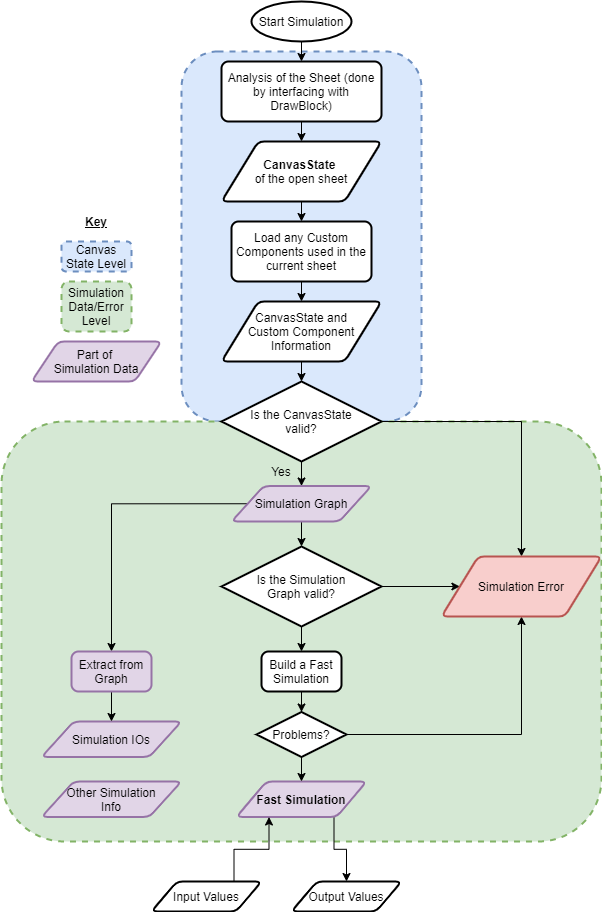
\includegraphics[width=\textwidth]{04.ImpPlan/IssieSim.png}
    \caption{An overview of Issie's Step Simulation}
    \label{fig:flowchartSim}
\end{figure}

\newpage % Here to ensure flowchart figure is in the right place

\subsection{Generating Truth Tables for a partial selection of a Sheet}
\emph{Associated Requirements:} \textbf{E1.2}, \textbf{E1.3}

The motivation behind Requirement \textbf{E1.2} is that a large schematic with lots of components will often contain smaller blocks of logic within it. These blocks may be defined Custom Components, or simply be a collection of gates in one corner of the canvas. Either way, there is value in the user being able to isolate these blocks and learn about the combinational logic implemented by them. Such functionality would also allow users to take a divide-and-conquer approach to debugging logical errors - individual blocks could be inspected to ascertain if they had been implemented correctly. 

A challenge with generating a truth table from part of a canvas is that Issie has no existing method for simulating part of a canvas. When working with a whole sheet, the inputs and outputs are well-defined; sheets where any ports aren't connected to inputs/outputs throw \textit{Simulation Errors}. In contrast, a partial selection from a sheet will rarely contain all inputs and outputs. Two methods were considered for simulating the selected logic to generate a truth table, with the latter being chosen.
\begin{enumerate}
    \item \textbf{Extracting the Fast Simulation and feeding values into specific wires}. This method would have involved creating a Fast Simulation for the whole sheet as usual, but then manually changing values in component arrays and seeing how those changes propagated through to the output connections of the selected logic. While this method seemed fit initially, several issues were found after some analysis. The Fast Simulation would be built for the whole sheet, meaning that an error elsewhere on the canvas would stop the selected logic from being simulated. Custom Components would also be harder to manage as the Fast Simulation datatype flattens the design, meaning that all nested logic in Custom Components would be expanded out. The new logic would also be quite different from the truth table generation logic for whole sheets - this is not ideal for future code maintenance purposes.
    \item \textbf{Intelligently building and correcting a new Canvas}. Following the highlighting of the issues with the first approach, an alternative approach was put forward. Rather than attempting to work with the complicated Fast Simulation data structure, it instead aims to use as much of the existing code as possible by treating the selected logic as a separate instance of a Canvas State and trying to simulate it using the same method as simulating a whole canvas. The main difference between simulating a whole sheet and simulating selected logic is the lack of guaranteed input and output components. This is overcome by finding which ports/connections are inputs/outputs for the selected logic, then intelligently adding 'phantom' input/output components to the canvas in a process called Canvas Correction. Once a corrected canvas corresponding to the selected logic is created, the logic used for generating and viewing a Truth Table for a whole sheet can be reused.
\end{enumerate}

Prior to the canvas correction stage, the selected components are checked. If only connections are selected, then a \textit{Simulation Error} is returned to the user informing them of their mistake.

\subsubsection{Canvas Correction}
\begin{itemize}
    \item[Step 1] \textbf{Add Extra Connections:} Sub-figures \ref{subfig:SelCase2} to \ref{subfig:SelCase4} in Figure \ref{fig:SelCases} all show situations where one or more inputs/outputs for the selected logic are ports on components, rather than connections. Taking the case shown in Figure \ref{subfig:SelCase2} in particular, the inputs to the selected logic are: both input ports on G1, and the bottom input port on G2, while the outputs from the selected logic are both output ports on G1 and G2 respectively. Prior to correction, the selection canvas does not have any connections going into those ports. This step finds any ports on selected components which do not have a connection in the selection and connects them to "dummy" input or output ports depending on their \codestyle{PortType}. This transforms the canvas to a state similar to that seen in Case (a), where   all inputs into the selected logic have connections.
    \item[Step 2] \textbf{Add Extra IOs:} This step adds the "phantom" input and output components to the selection canvas. The locations where these components need to be inserted are found by checking which connections in the Canvas State do not have both ports present in the selection. Any such connections are either connected to some other component in the sheet which is not selected, or are newly added connections which are connected to dummy ports. Either way, these are the connections that need to be connected to "phantom" IOs. 
    \begin{itemize}
        \item[Step 2.1] \textbf{IO Width Inference:} When creating new input or output components, the correct width must be specified. This is         calculated by running Issie's \codestyle{WidthInferrer} on the whole sheet to find the expected width of the input or output. However, in cases such as the one shown in Figure \ref{subfig:SelCase4}, where there are no connections to/from some ports on G3, \codestyle{WidthInferrer} will fail to infer widths, resulting in a \textit{Simulation Error}. A possible workaround would be to try to infer the width from the component itself if \codestyle{WidthInferrer} fails - in Issie AND gates always have 1-bit inputs, so any "phantom" inputs generated would have a width of one. This would be trivial to implement in the future. However, there would still be cases, such as inputs into multiplexers and n-bit XORs, where even this approach would not work.
        \item[Step 2.2] \textbf{IO Label Inference:} Usually users provide labels for IOs, which are used in the Truth Table. However, when IOs are automatically created, names for them must be automatically generated too. This is done by looking at which ports in the selection they are connected to. The expression for an automatically generated IO Label is: \codestyle{[Connected Component Label]\_[IN/OUT][SUFFIX]}. If the port is labelled (e.g. on a multiplexer or a Custom Component), the suffix is the port label. Alternatively it is the \codestyle{PortNumber}, which indicates the position of a port on its host component.
        
    \end{itemize} 
    \item[Step 3] \textbf{Returning a Canvas or an Error:} If any errors were found in the previous steps, most likely due to a malformed selection, they are returned. If not, then the returned Canvas State is completely compatible with the existing simulation and truth table generation functions.
\end{itemize}

Following Canvas Correction, any returned Canvas State is fully compatible with the existing functions for simulating logic and generating truth tables. Therefore, a Truth Table can be generated for selected logic through the same methods and functions used for generating Truth Tables for the whole sheet.

\bigskip
\begin{figure} [h]
    \begin{subfigure}{0.48\textwidth}
        \centering
        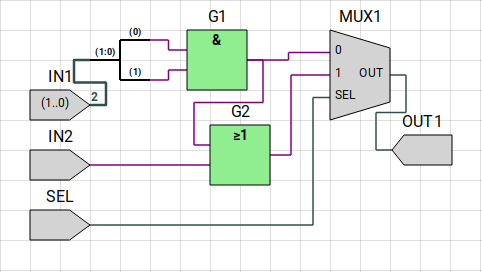
\includegraphics[width=0.8\linewidth]{04.ImpPlan/SelCase1.png}
        \caption{Case where all inputs into selected logic are connections.}
        \label{subfig:SelCase1}
    \end{subfigure}
    \begin{subfigure}{0.48\textwidth}
        \centering
        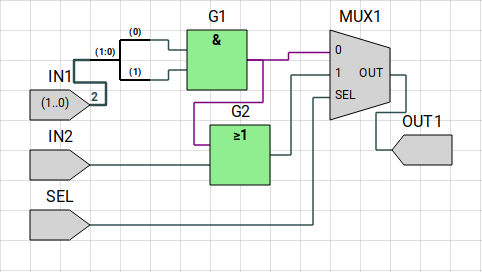
\includegraphics[width=0.8\linewidth]{04.ImpPlan/SelCase2.png}
        \caption{Case where some inputs into selected logic are connections, and some are ports on components.}
        \label{subfig:SelCase2}
    \end{subfigure}
    \newline
    \begin{subfigure}{0.48\textwidth}
        \centering
        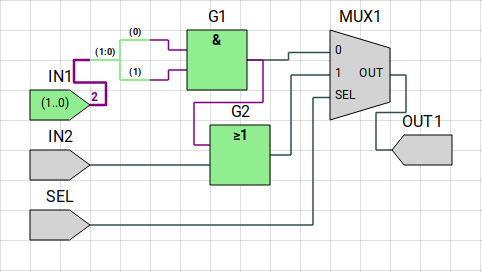
\includegraphics[width=0.8\linewidth]{04.ImpPlan/SelCase3.png}
        \caption{Case where selected logic includes an input component.}
        \label{subfig:SelCase3}
    \end{subfigure}
    \begin{subfigure}{0.48\textwidth}
        \centering
        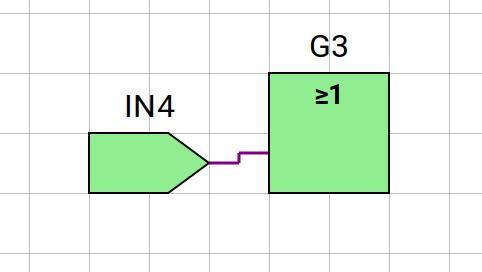
\includegraphics[width=0.8\linewidth]{04.ImpPlan/SelCase4.png}
        \caption{Case where a selected component does not have connections to all ports}
        \label{subfig:SelCase4}
    \end{subfigure}
    \caption{Selection Cases}
    \label{fig:SelCases}
\end{figure}

\subsection{UI Changes}
\emph{Associated Requirements:} \textbf{D3.1}
As mentioned in Section \ref{sec:IssieUI}, there are inconsistencies in Issie's current UI, particularly concerning the Waveform Simulator. With the addition of Truth Table viewing to Issie, the decision was made to tweak the UI to try to keep everything consistent. Figures \ref{fig:OldUI} and \ref{fig:NewUI} show the old and newly tweaked UIs respectively. The top bar primarily houses operations or information concerning files, such as the button to save the sheet, menu to open other sheets/projects, and the filepath. As a result the \textit{Waveforms} button has been removed from there. Ideally it would have a permanent place on the right tab, however with the addition of a Truth Table tab this would take the total number of tabs up to five, causing the tab label text to become illegible.  Given that there are now three ways to gain an insight into the logic on the sheet (Step Simulator, Truth Tables, Waveform Simulator), it is logical to group these together as sub-tabs under one main tab. The new UI now always has three tabs on the right in contrast to the old UI which would spawn the WaveSim tab when viewing Waveforms. Clicking the right-most "Simulations" tab will now reveal three sub-tabs: Step Simulation, Truth Tables, and Wave Simulation. The behaviour of the Truth Table view and the updated WaveSim view is modelled on that of the Step Simulator. Selecting a tab for the respective simulator will reveal a short description of the function, and a button to start the appropriate action. The colour and message shown by this button is dependent on the sheet: problems will show a yellow button, and a solid green button shows that the sheet is correct, and the functionality is available. Light green means that while the sheet is syntactically correct, some other factor is making the functionality unavailable. For the Waveform simulator this is when the sheet contains no synchronous logic (meaning no waveforms to display), and for Truth Tables it is when the sheet does contain synchronous logic (as synchronous logic is currently not supported for truth tables).

\begin{figure}
    \centering
    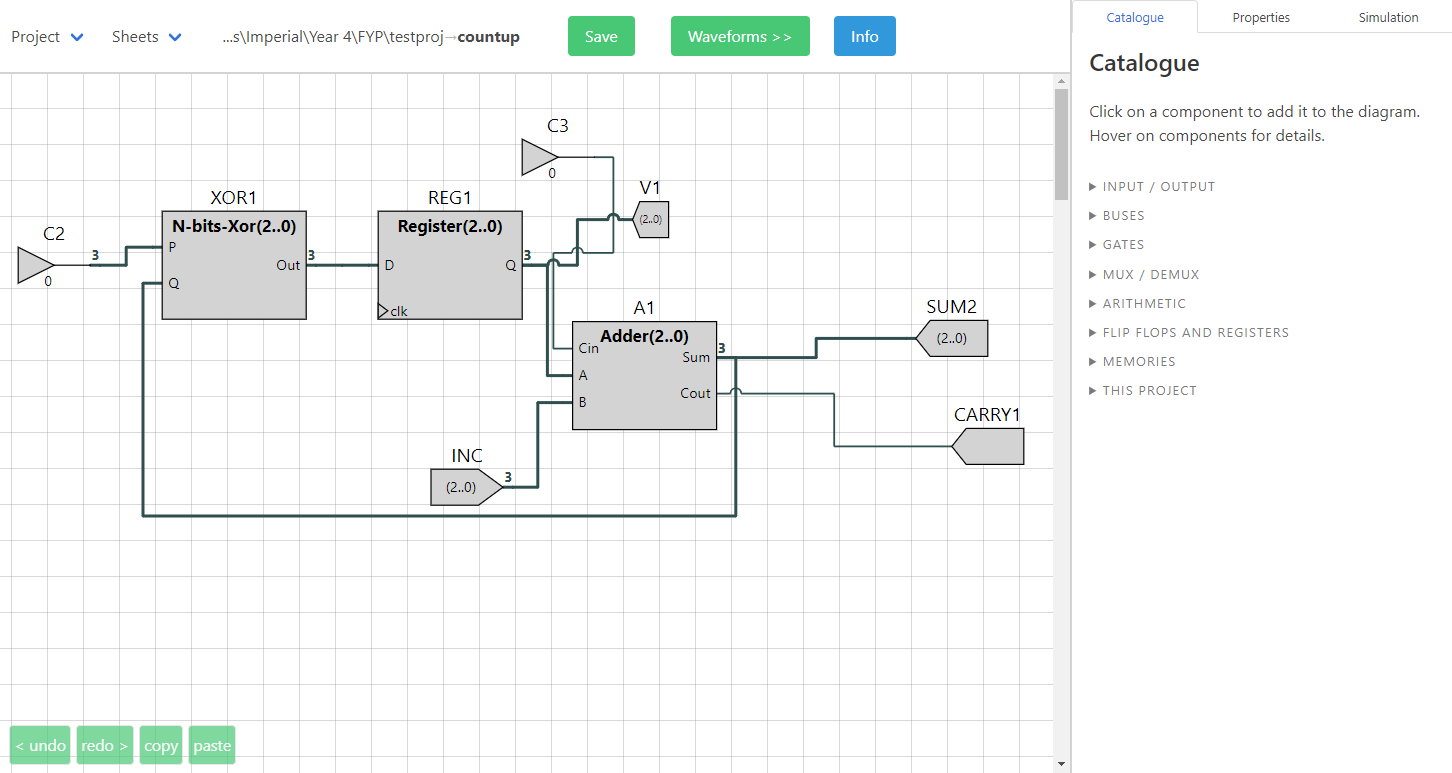
\includegraphics[width=0.8\textwidth]{04.ImpPlan/OldUI.png}
    \caption{Old Issie UI}
    \label{fig:OldUI}
\end{figure}

\begin{figure}
    \centering
    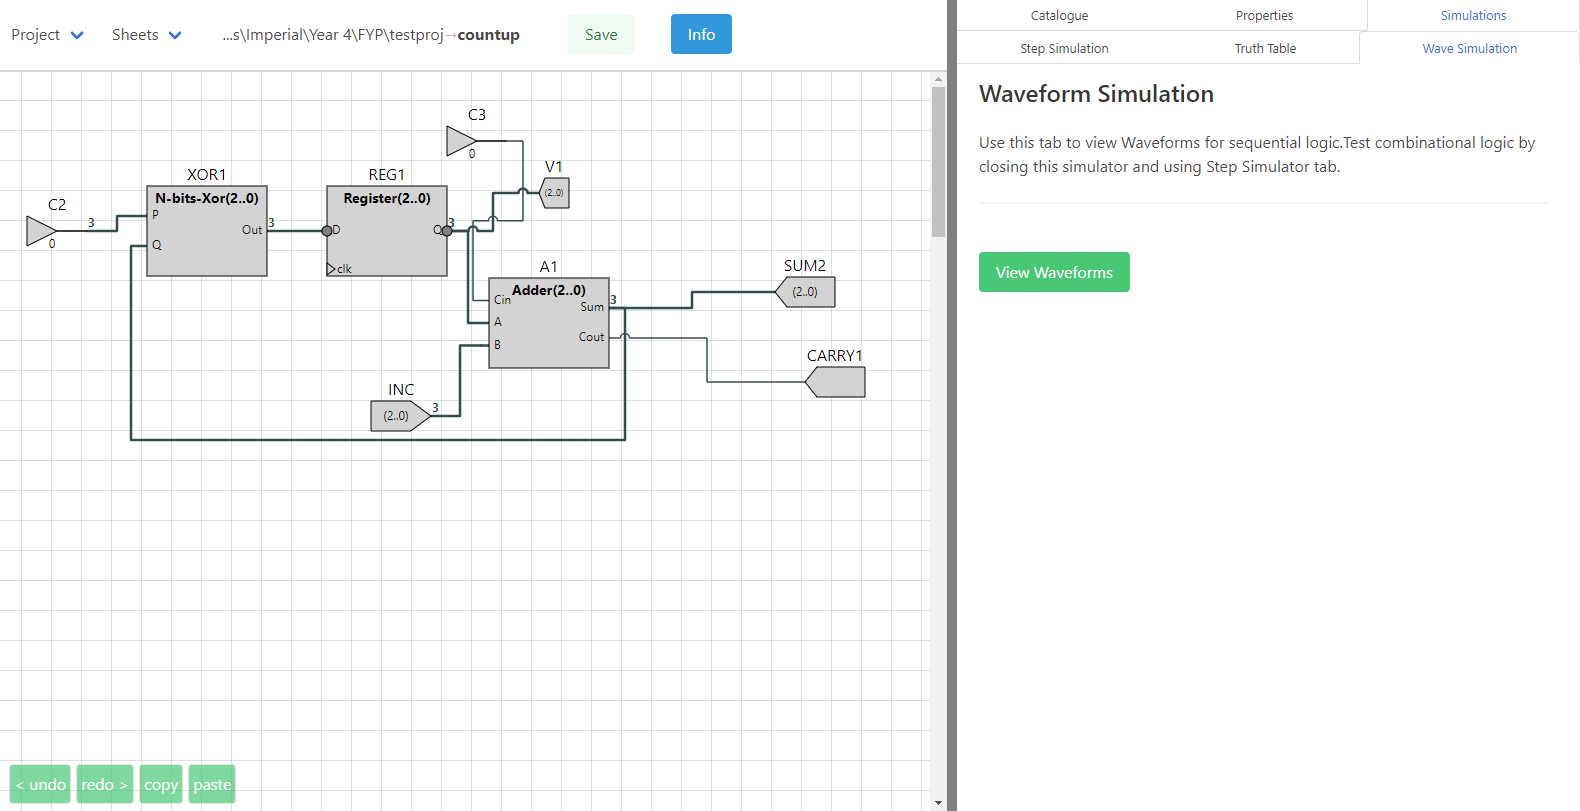
\includegraphics[width=0.8\textwidth]{04.ImpPlan/NewUI.png}
    \caption{New Issie UI}
    \label{fig:NewUI}
\end{figure}

\section{Work Breakdown Structure}
As with any large project, a key stage in planning is to break it down into several manageable chunks. This has been done to some extent in the Requirements Capture (Chapter \ref{chap:requirements}), albeit at quite a high level. On the other hand, a Work Breakdown Structure (WBS) \cite{projectmanagement} defines the scope of the project and breaks the work down into components that can be scheduled, monitored, and controlled. This aids in assessing the complexity of certain tasks, therefore improving the overall distribution of resources (mainly time) to different tasks. The WBS for this project is shown in Figure \ref{fig:wbs} - it is rotated to make it more clear to the viewer. Red nodes in the WBS could be considered as \emph{Initiatives}, as they are long term (relative to the length of the project) objectives. Green nodes are rough equivalents to \emph{Epics}, and white/grey nodes are \emph{User Stories}. In some cases, user stories may have very short sub-tasks underneath them which need not necessarily be differentiated, but are done on the WBS for clarity's sake. User Stories which spawn sub-tasks are coloured purple, while sub-tasks requiring further elaboration are coloured yellow. 

\section{Time Management and Gantt Chart}
Effective time management is vital to any project; traditionally a Gantt chart is used to display the timeframe in which the tasks detailed in the WBS will be completed. In line with this, a Gantt chart has been prepared for this project, and can be seen in Figure \ref{fig:gantt}. The colour coding on the chart matches that on the WBS, and key deadlines are indicated by dashed vertical lines. The first line represents the Interim report deadline - therefore any work shown on the chart to the left of this line is already completed, while any work to the right of the line is planned. The layout of Figure \ref{fig:gantt} allows it to double as a chronologically structured backlog. Within Initiatives, Epics are placed in chronological order, and likewise for User Stories within Epics. Two main considerations were made when devising this order of items. Firstly, dependencies were considered - for example it would be foolish to write code to view truth tables prior to there being a mechanism to generate them. Secondly, the importance of the deliverable associated with a task was taken into account - with tasks that fulfilled essential requirements given precedence over those that fulfilled desired requirements. 

\subsection{Contingencies and Strategies taken to Mitigate Risk}
The project plan has been structured to contain a healthy contingency allowance. Looking at the order of work in the Gantt chart, it can be seen that all essential requirements (and the majority of the desired features) should be fulfilled by the beginning of May. Furthermore, all technical work is expected to be completed by the end of May, bar a possible need to reconfigure parts of Issie's overall GUI (which is very unlikely).
Additionally, most time estimations for tasks have some margin built in as well, reducing the likelihood of technical work overrunning. This leaves the last three weeks of the project dedicated solely to report writing and documentation; two tasks which ideally will have been worked on over the duration of the project. Therefore, this plan yields a contingency allowance of three weeks.
The project management strategy, formed by a fusion of plan-based and Agile management methods, also acts as a form of contingency. As stated, the backlog ordering methodology has taken into account dependencies and importance of deliverables. If progress is slow, then the backlog can be dynamically reorganised, with less essential items shifted or removed. The ultimate fallback is to only implement the essential features, but such an extreme case is highly unlikely to arise. On the other hand, if progress runs ahead of schedule extension tasks can be discussed.

\begin{figure}
    \centering
    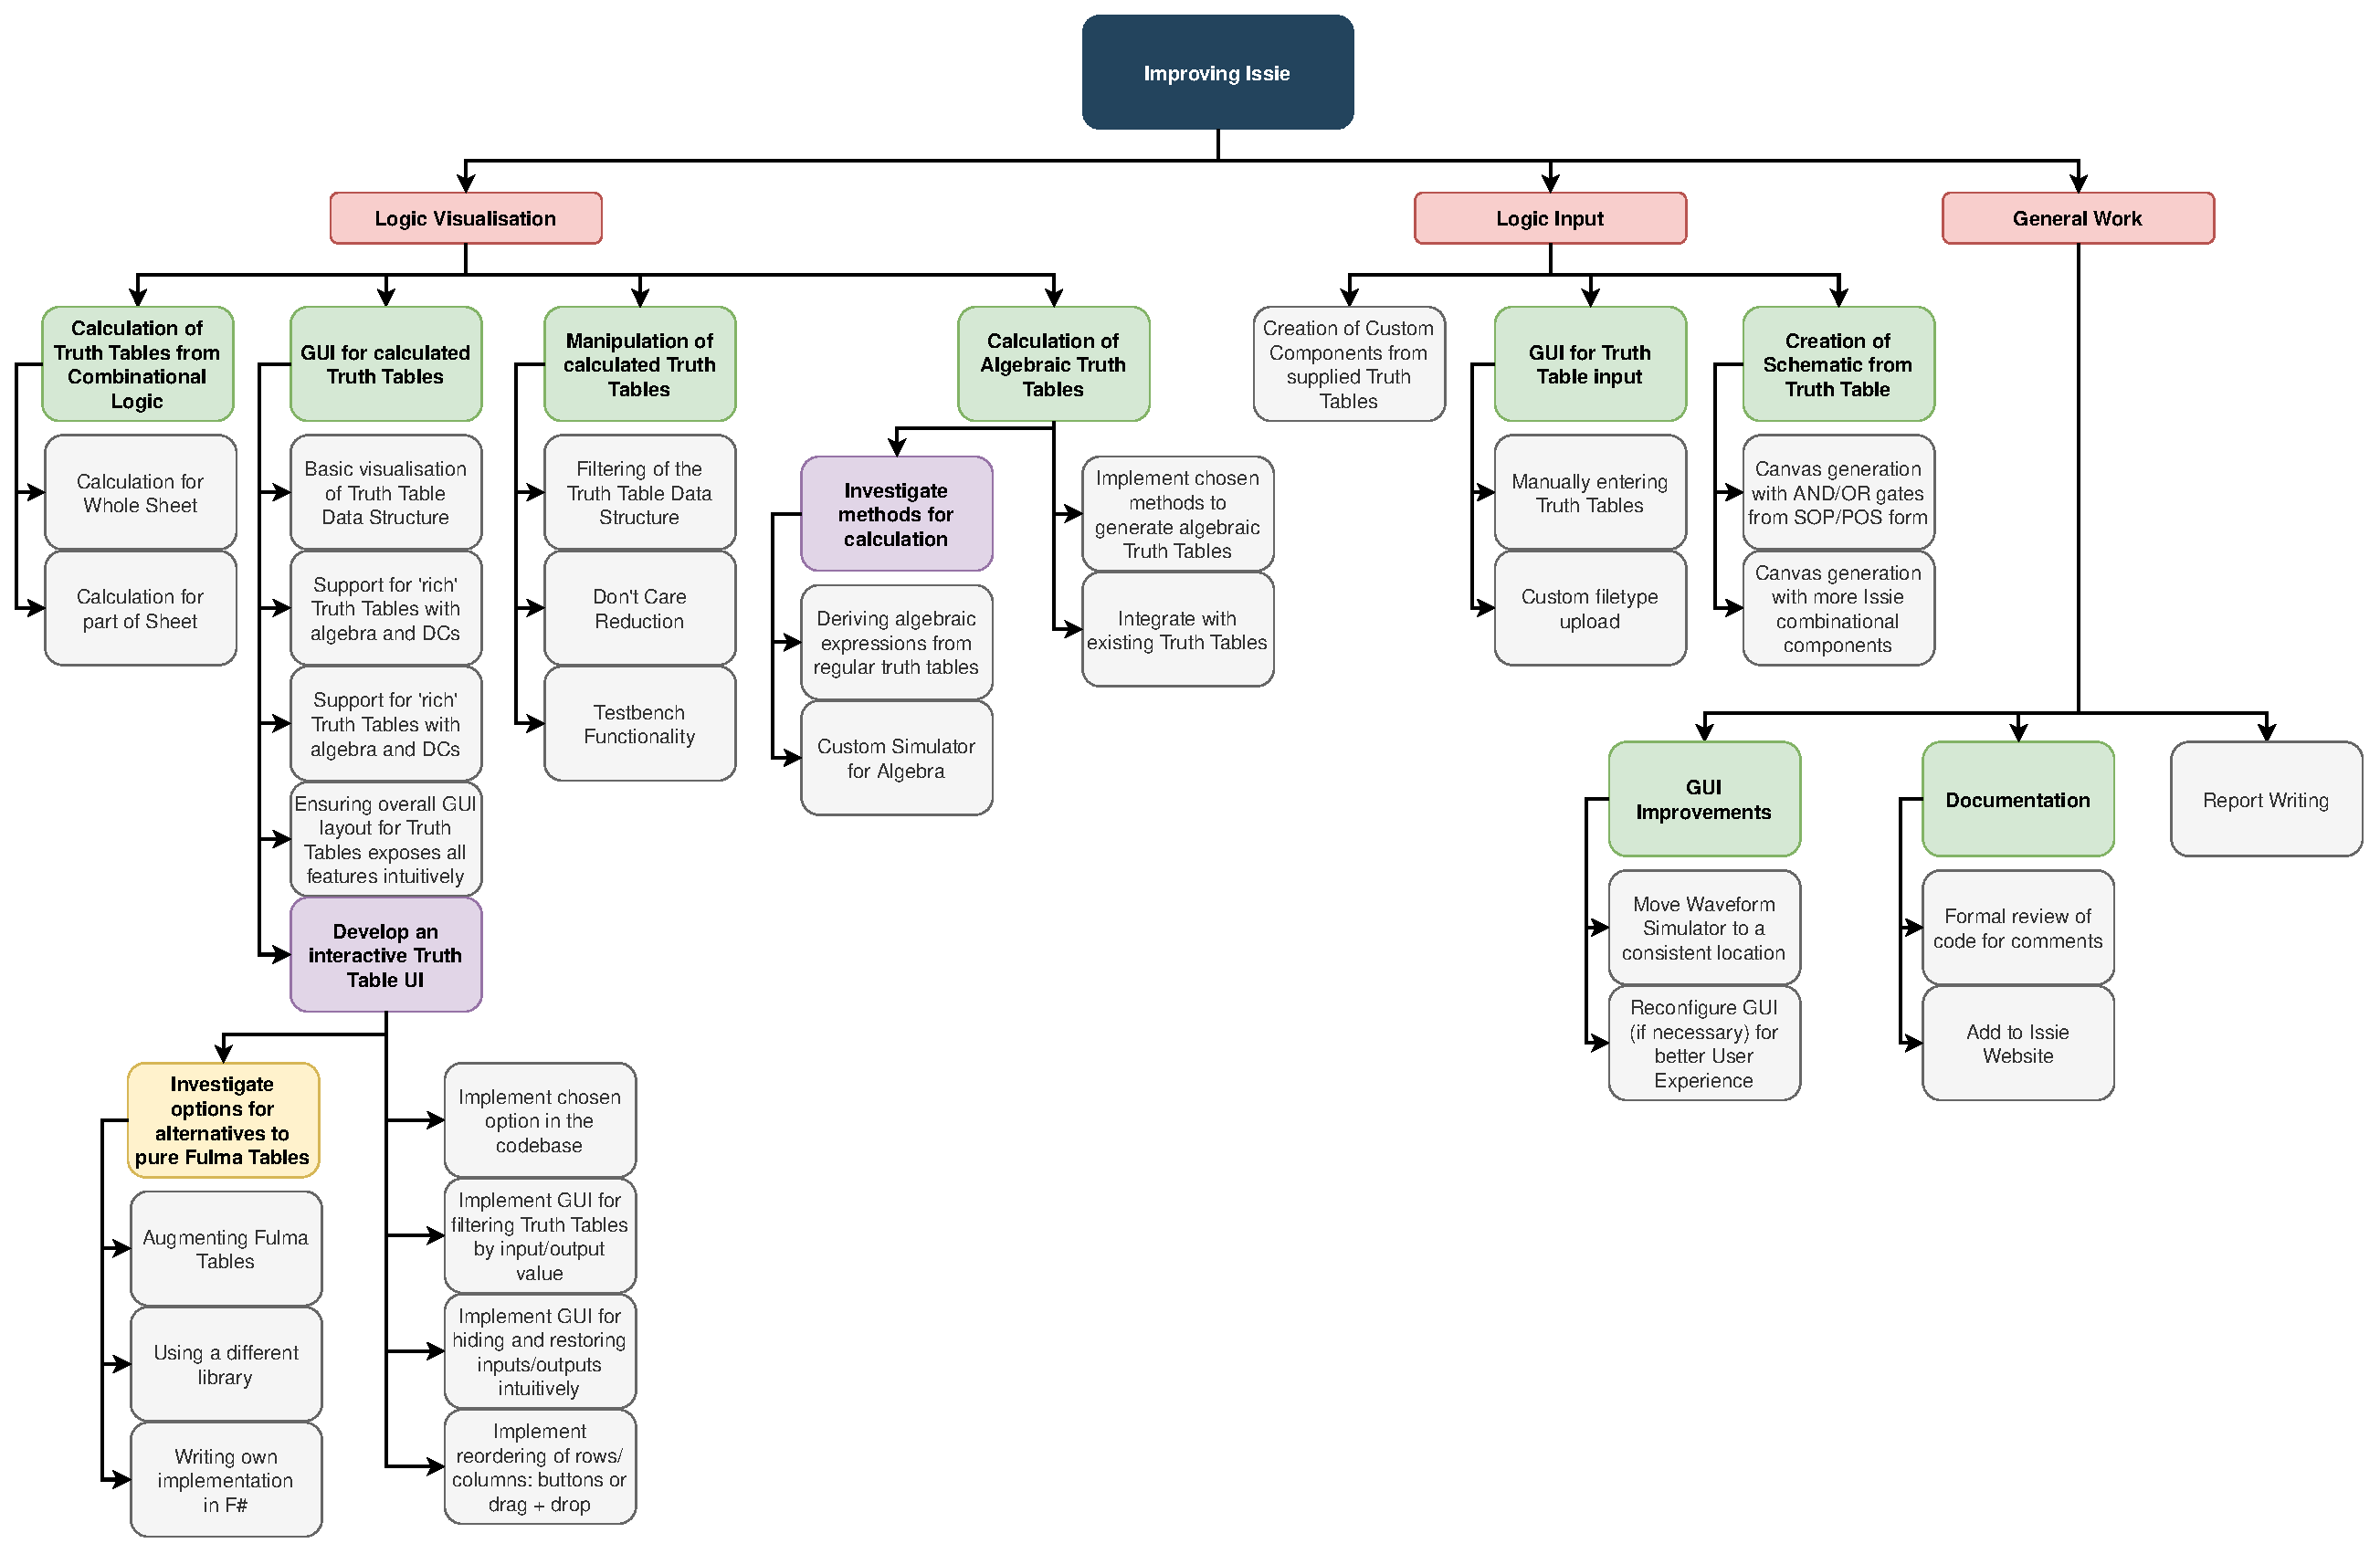
\includegraphics[width=22cm,angle=270,origin=c]{04.ImpPlan/wbs.eps}
    \caption{Work Breakdown Structure for the Project (Rotated)}
    \label{fig:wbs}
\end{figure}

\begin{figure}
    \centering
    \includegraphics*[width=\textwidth]{04.ImpPlan/gantt_update.pdf}
    \caption{Gantt Chart for the Project}
    \label{fig:gantt}
\end{figure}
\chapter{Evaluation Plan}
This project has two main deliverables; an extended and improved version of Issie, and any appropriate documentation for the application. These deliverables will be evaluated against a series of metrics, both qualitative and quantitative.
\section{Evaluation against Requirements}
The bare minimum expectation of the project is that it \textbf{must} fulfil all Essential Requirements outlined in the Requirements Capture (Chapter \ref{chap:requirements}). Anything less than this would suggest that the project was not successful in achieving its goals. The only exception to this would be that if, during the development process, a feature outlined by a requirement was deemed to be unnecessary and therefore changed. The success of the project will also be measured on how many of the Desired Features are fulfilled, with the ideal scenario being that all requirements are satisfied. 

Most of the outlined requirements are features that the final deliverable should incorporate. Therefore, these requirements can simply be evaluated by opening the application and testing that they work as intended. The correctness of such features can be tested by opening existing Issie schematics featuring various circuits built by users, and checking if the added features perform as expected when used on those sheets. Additionally, testing will occur throughout the development process - each feature will be unit tested prior to its integration to Issie. 
In contrast to the type mentioned above, certain requirements cannot be objectively judged as complete, such as those related to intuitiveness of the UI. The subjective nature of such requirements mandates that their satisfaction be evaluated by multiple end-users. Therefore, the chosen evaluation methods for Requirements \textbf{E1.6}, \textbf{E1.7}, and \textbf{D3.1} will be a survey answered by volunteers who have spent time using the delivered application to perform a series of basic tasks.

\section{Overall Evaluation}
The overall aim of the project is to improve Issie as a digital electronics education tool and as a logic design application. The effectiveness of the features this project will add must be judged by those who stand to benefit from them - the user base. Therefore, the survey mentioned in the previous section will also include questions on if the newly added features helped them in designing the logic specified in the tasks. For one task in the survey the group will be split into two teams, with one using the original version of Issie and the other the one delivered by this project. The students will be given a series of custom components which implement increasingly complex, but still identifiable logic. The students will be asked to use Issie to identify which actual component the custom component implements using the tools their version of Issie provides them. The amount of time it takes them to reach an answer, and the correctness of that answer, will contribute to their score. The correlation between scores and Issie version will be observed and used to evaluate the version of Issie delivered by this project.

\printbibliography

\chapter{Appendices}

\section{Appendix A - Screenshots of Issie 2.4.0}
Screenshots taken on Mac.

\begin{figure} [h]
    \centering
    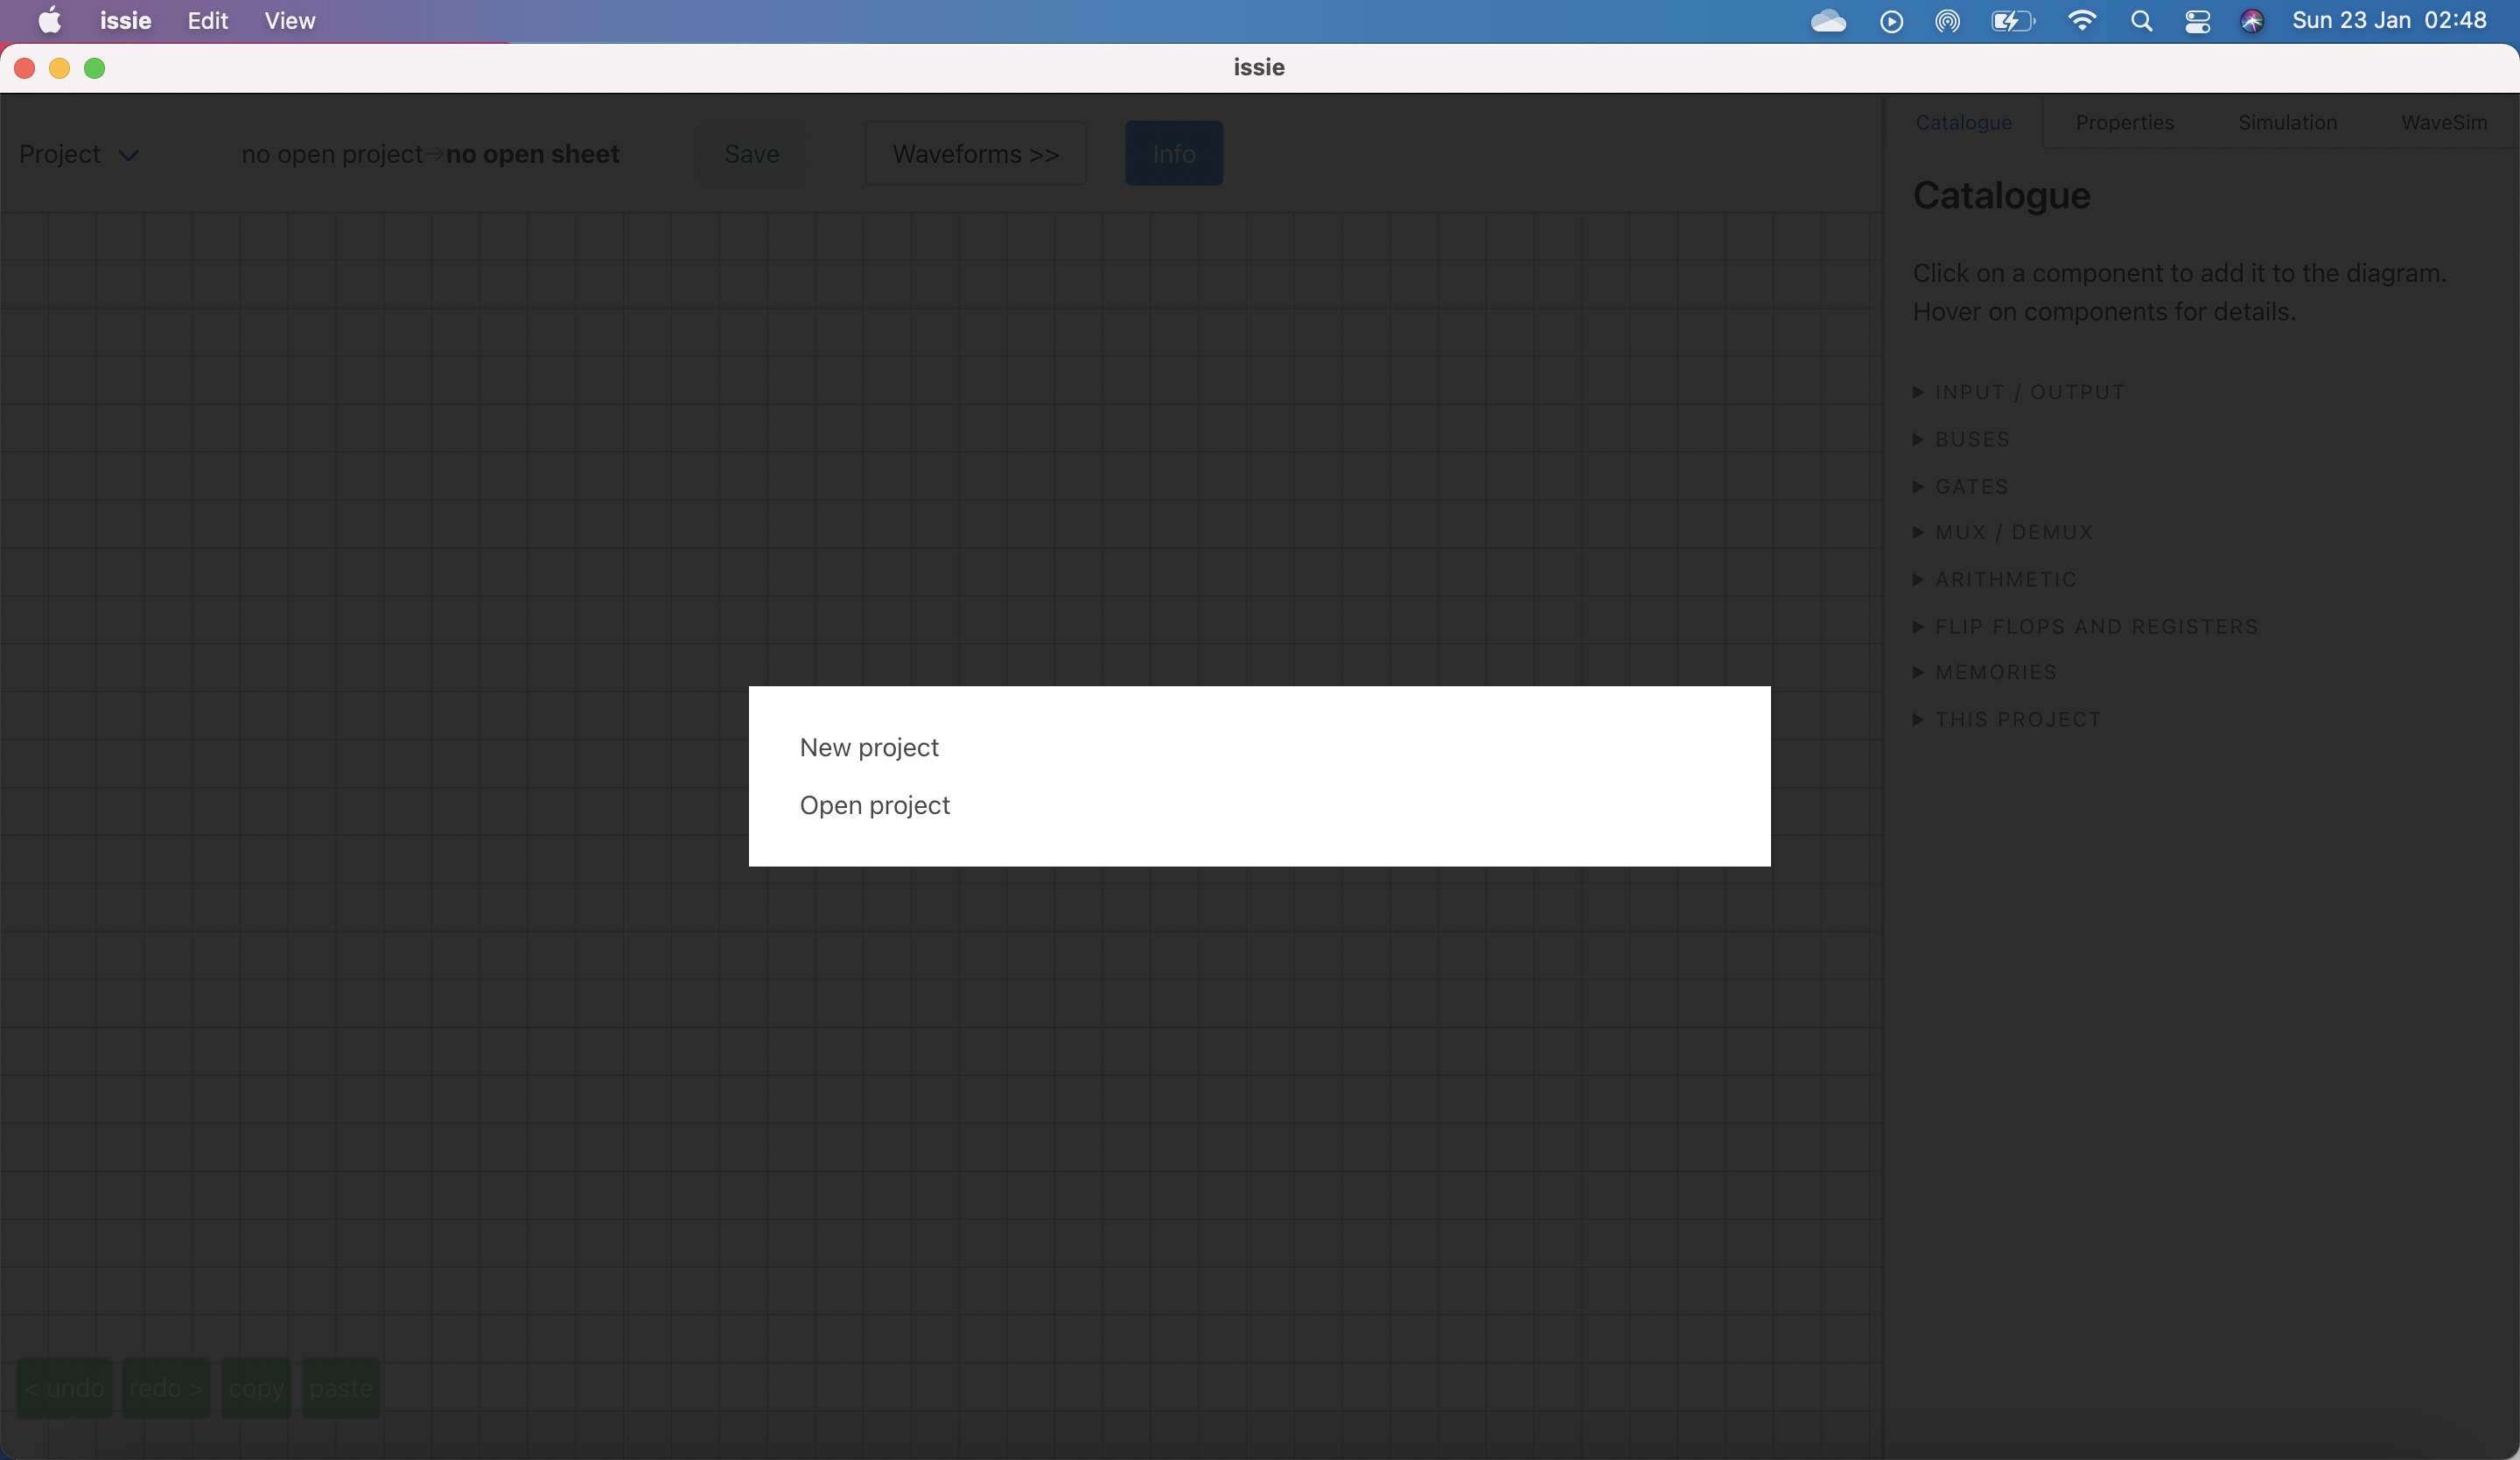
\includegraphics[width=\textwidth]{Appendices/IssieOpening.png}
    \caption{Issie's opening screen}
    \label{fig:IssieOpen}
\end{figure}

\begin{figure} [h]
    \centering
    \includegraphics[width=\textwidth]{Appendices/IssieSheetAnnotated.png}
    \caption{A sheet (schematic) open in Issie, with a component and wire selected}
    \label{fig:IssieSheetAnnotated}
\end{figure}

\begin{figure} [h]
    \centering
    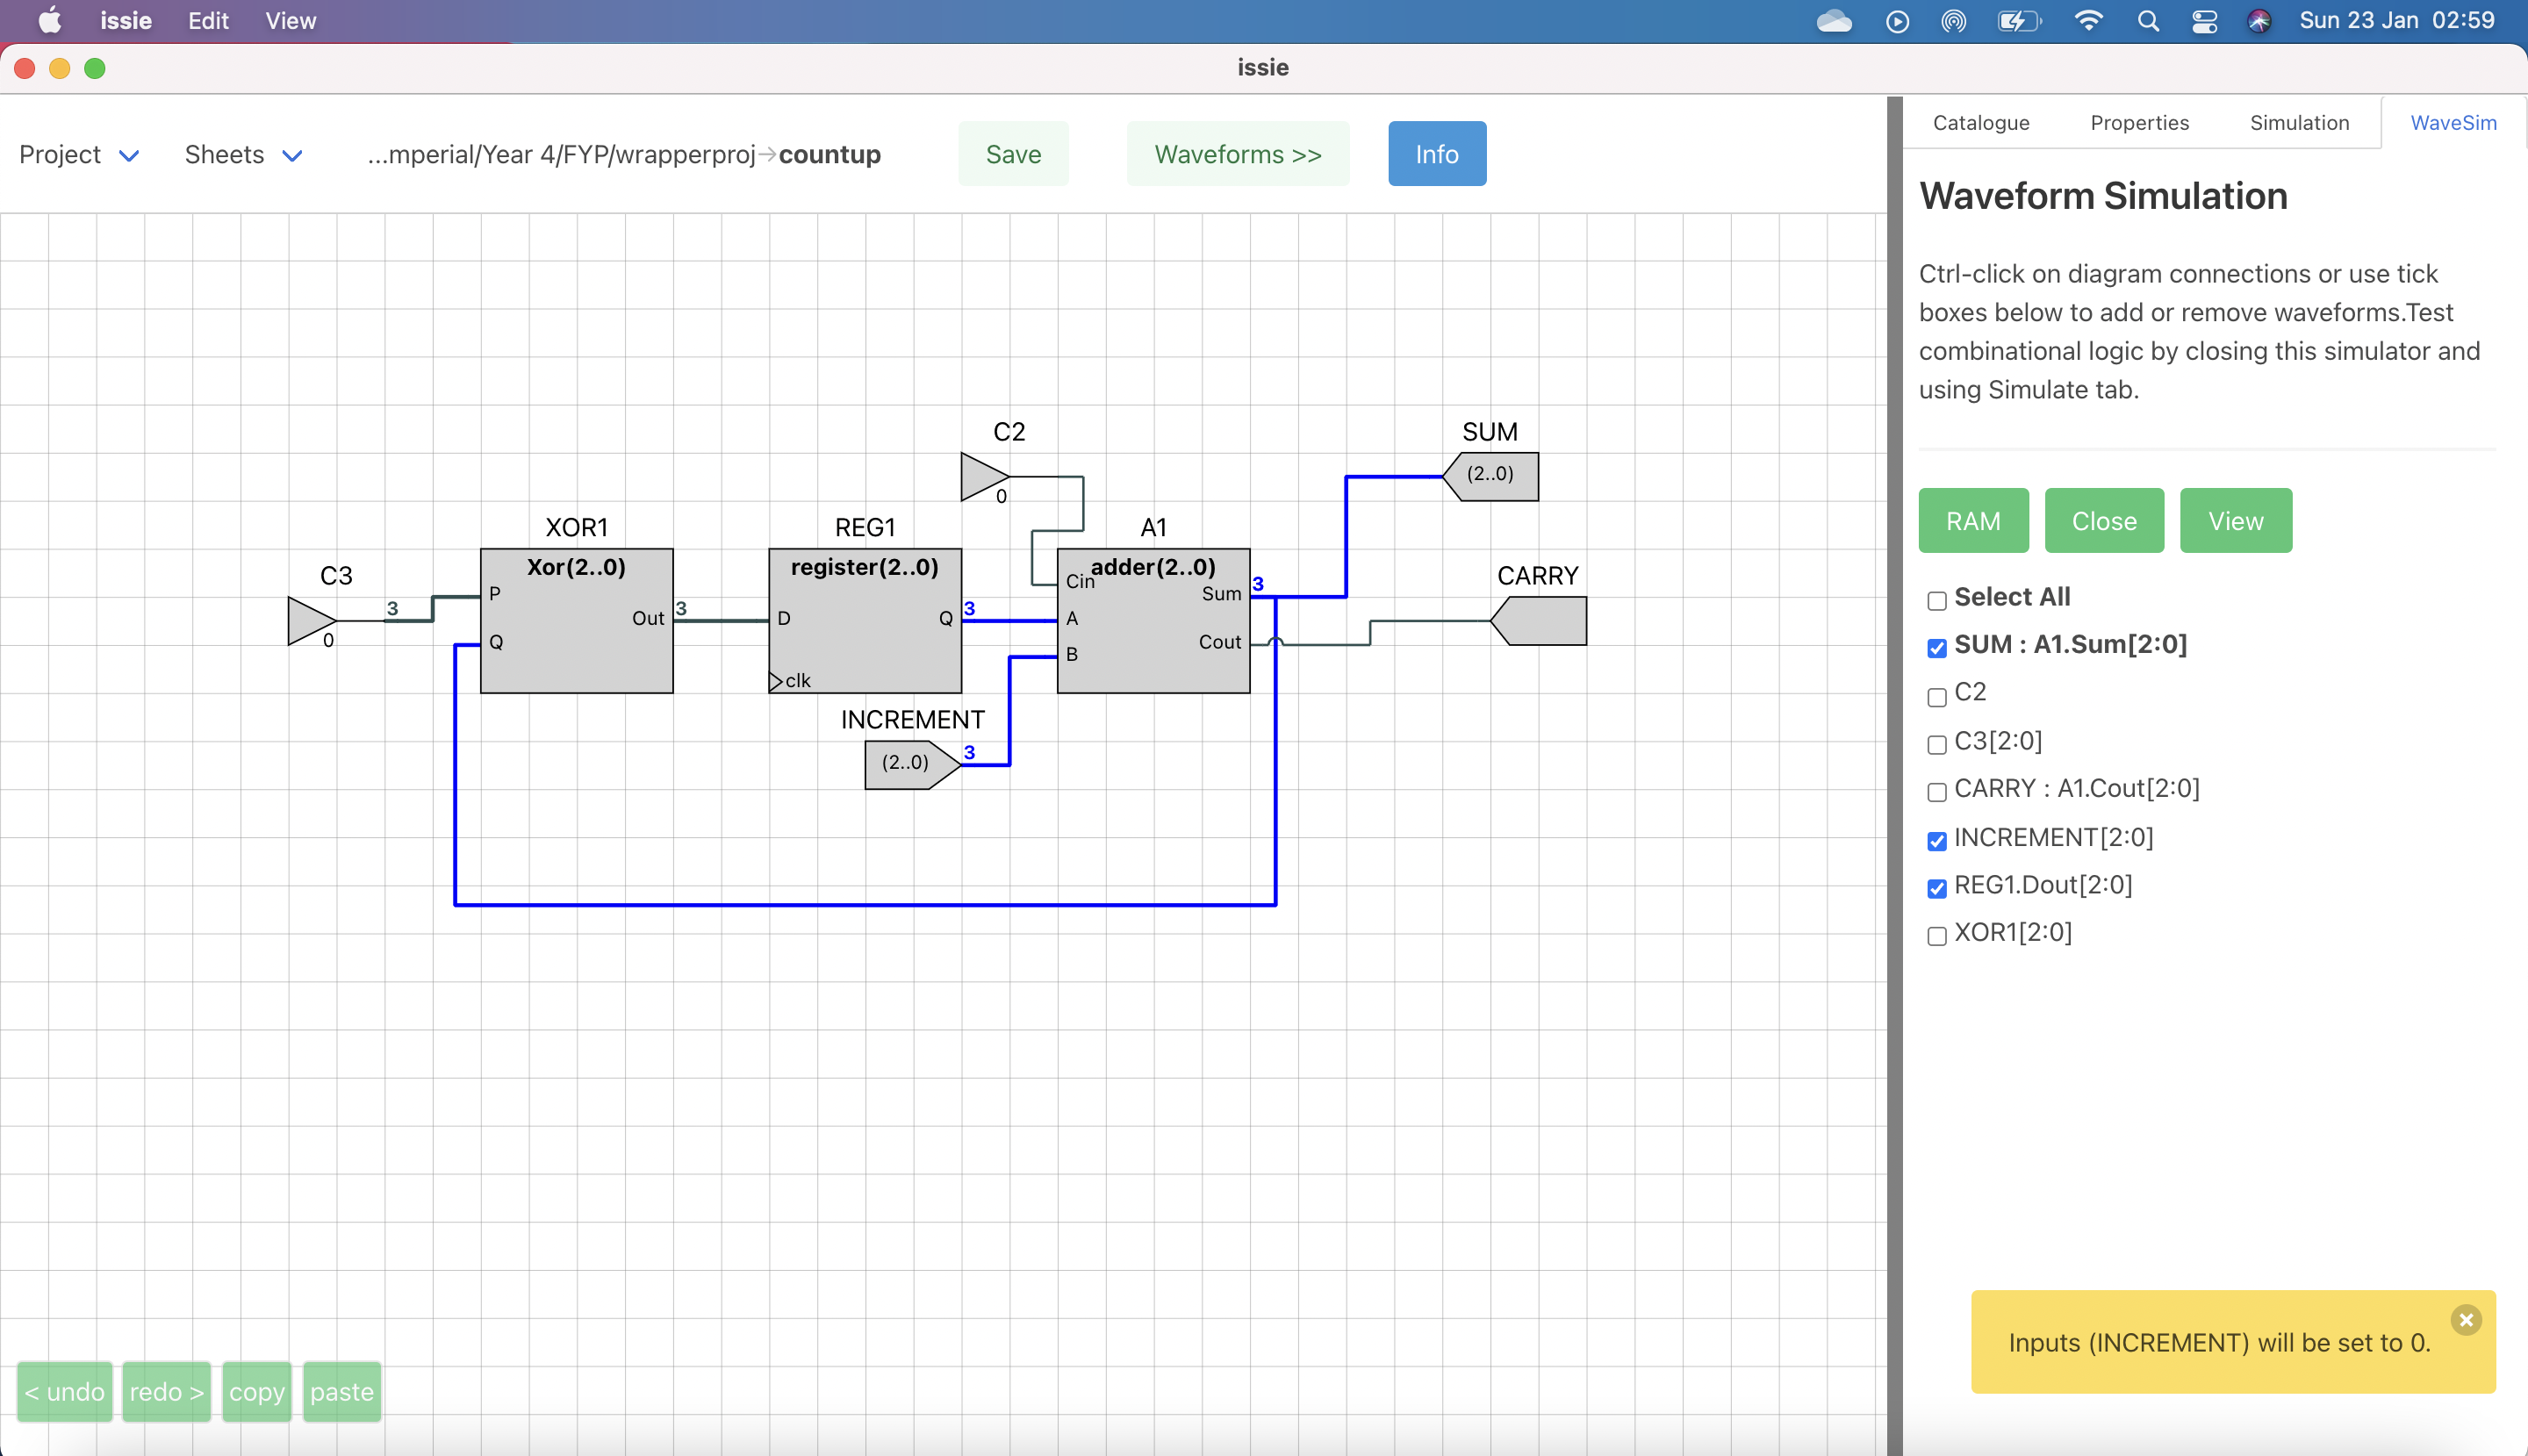
\includegraphics[width=\textwidth]{Appendices/IssieWaveSimSel.png}
    \caption{Issie's Waveform Simulator selection menu}
    \label{fig:IssieWSSel}
\end{figure}

\begin{figure} [h]
    \centering
    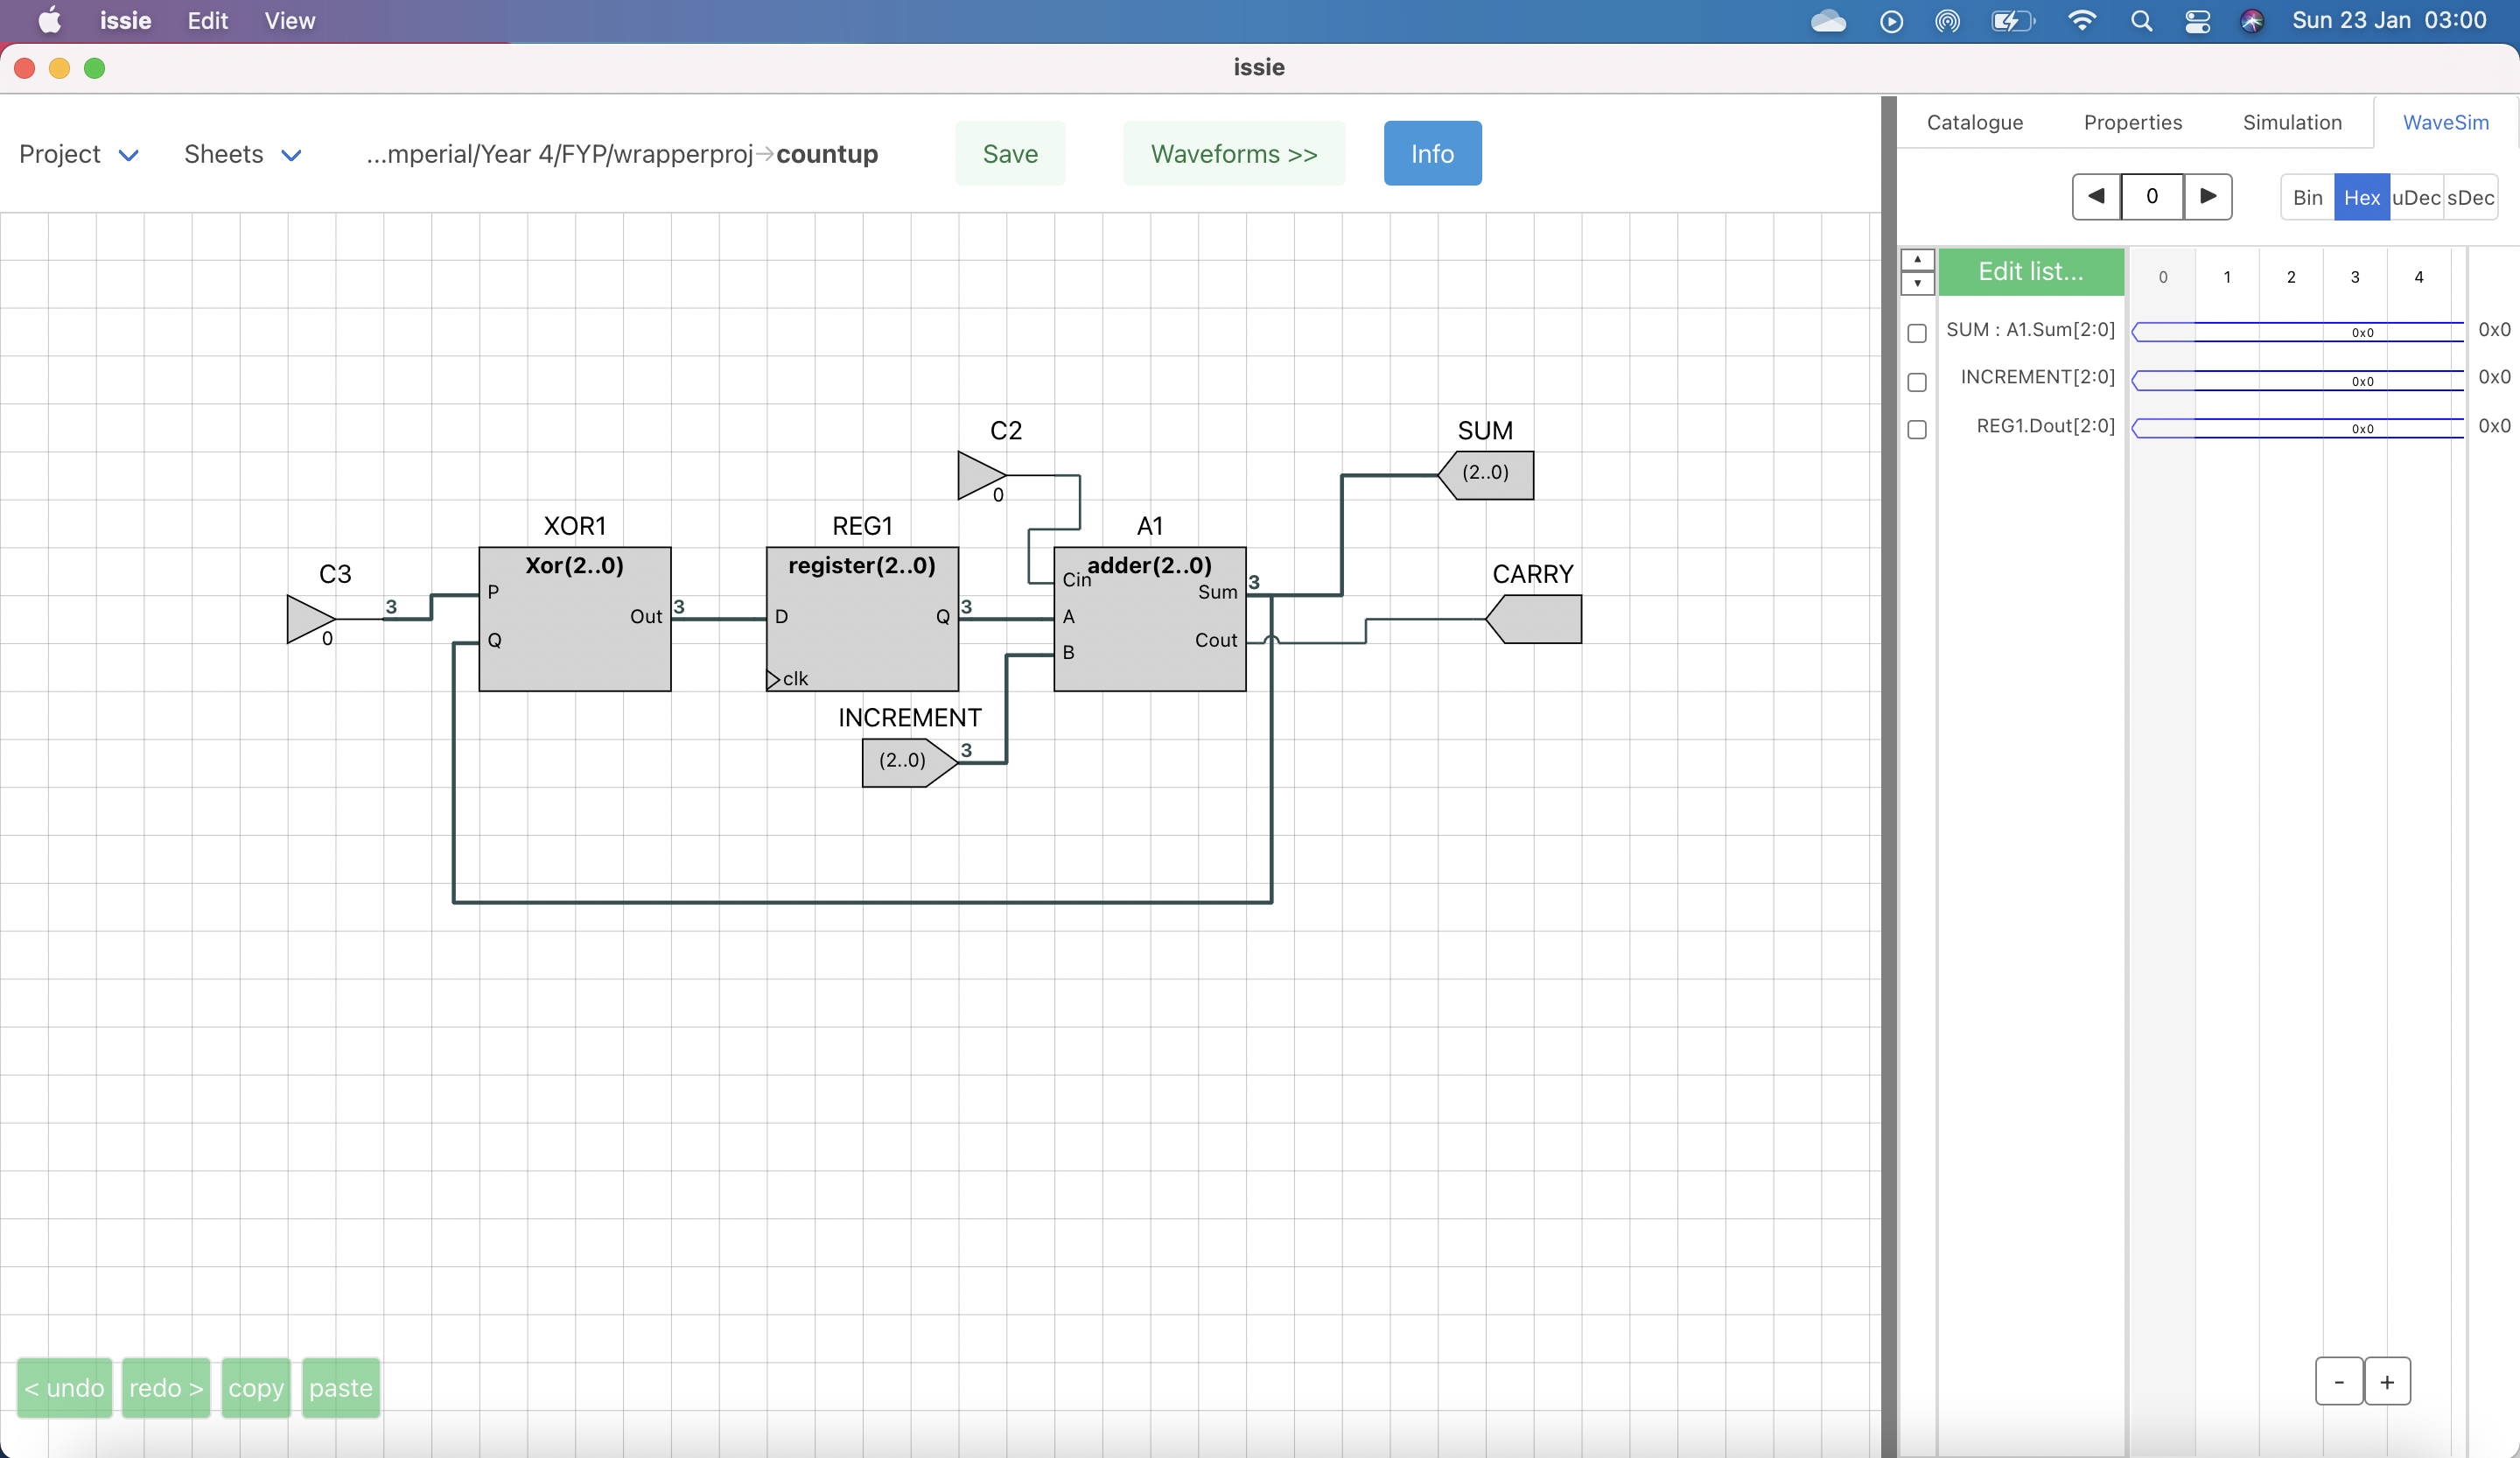
\includegraphics[width=\textwidth]{Appendices/IssieWaveSim.png}
    \caption{Issie's Waveform Simulator}
    \label{fig:IssieWS}
\end{figure}


\end{document}
